\begin{figure*}[h!]
	\begin{center}
		\hspace*{-.4in}
		\vspace*{-0.3in}
		\begin{tabular}{   c | c  c  c  c  }
			%\hline
			& \large{\textsf{VIDEO 1 }} &\large{\textsf{VIDEO 2}}   &\large{\textsf{VIDEO 3}} &\large{\textsf{VIDEO 4}}      \\ 
			&\vspace{-.1in}&&&\\
			& \large{\textsf{Pure Rotation}} &\large{\textsf{Rotating Hotspot}}   &\large{\textsf{Face-on Disk}} &\large{\textsf{Edge-on Disk}}      \\ \hline
			&\vspace{-.1in}&&&\\
			\multirow{1}{*}[0.9in]{ \rotatebox[origin=t]{90}{\small{\textsf{SINGLE FRAME}} }}
			&
			{{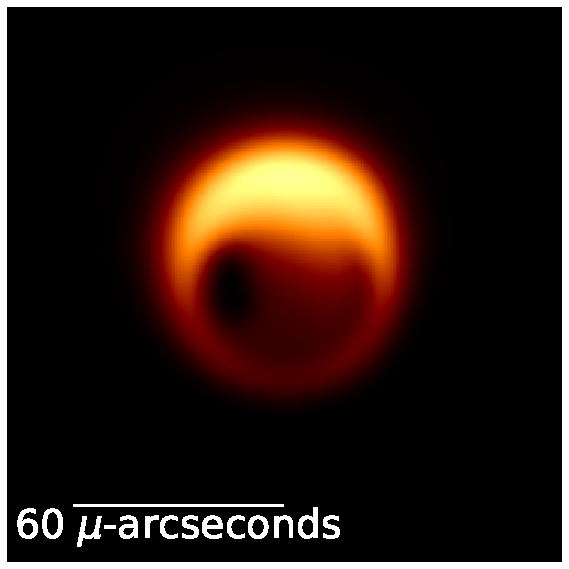
\includegraphics[height=.15\linewidth]{figures/starwarps_results/rotation30/gt/frames/gt_15_colorbar.pdf}} } 
			\multirow{2}{*}[.9in]{ 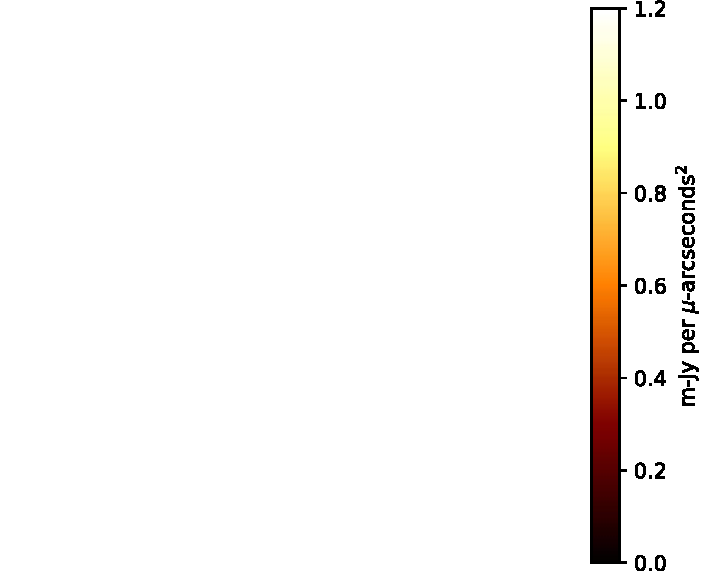
\includegraphics[width=0.06\linewidth]{figures/cbar/vertical_cbar_0to12.pdf} }
			&
			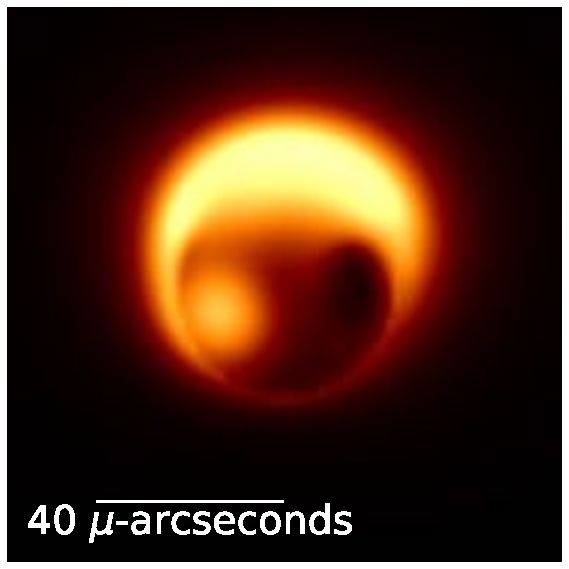
\includegraphics[height=.15\linewidth]{figures/starwarps_results/hotspot100sR2/gt/frames/gt_115_colorbar.pdf} 
			\multirow{2}{*}[.9in]{ 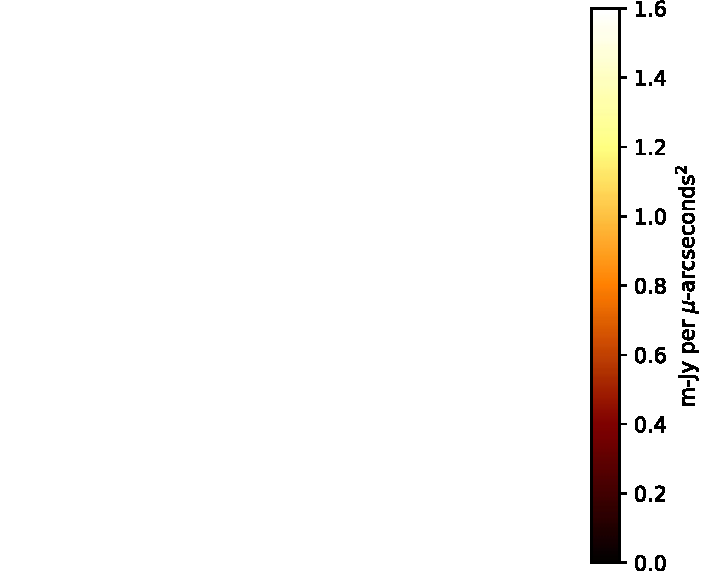
\includegraphics[width=0.06\linewidth]{figures/cbar/vertical_cbar_0to16.pdf} }
			&
			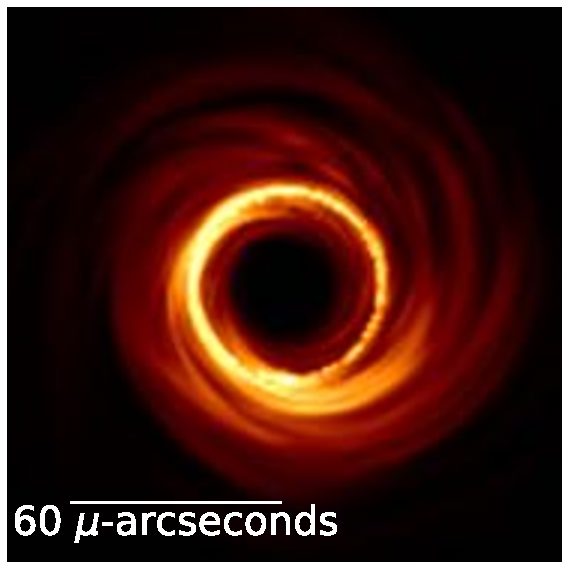
\includegraphics[height=.15\linewidth]{figures/starwarps_results/hotakamovie_02/gt/frames/gt_85_colorbar.pdf} 
			\multirow{2}{*}[.9in]{ 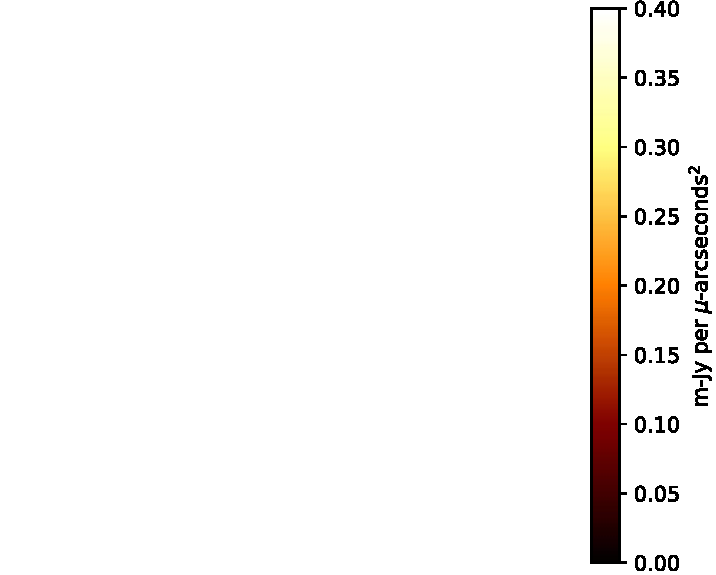
\includegraphics[width=0.0668\linewidth]{figures/cbar/vertical_cbar_0to4.pdf} }
			&
			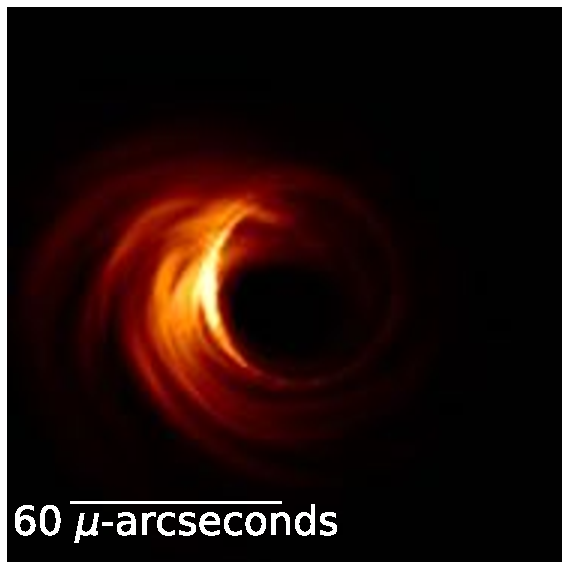
\includegraphics[height=.15\linewidth]{figures/starwarps_results/hotakamovie_45/gt/frames/gt_63_colorbar.pdf} 
			\multirow{2}{*}[.9in]{ 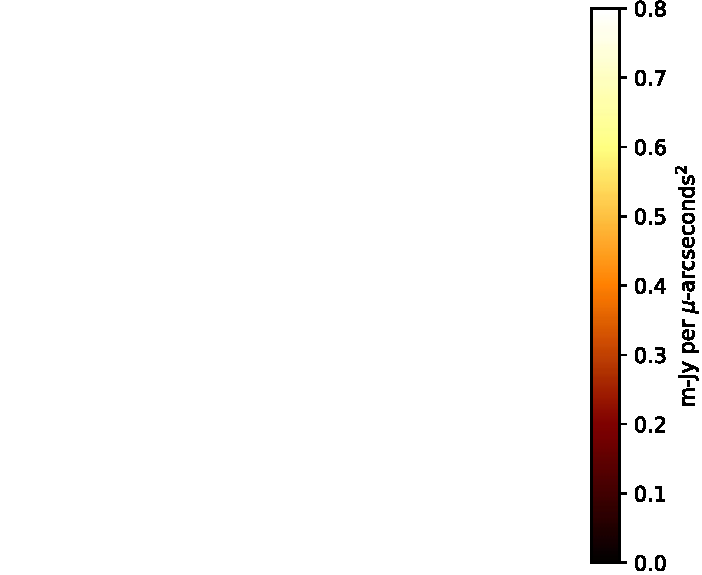
\includegraphics[width=0.06\linewidth]{figures/cbar/vertical_cbar_0to8.pdf} }
			\\
			\multirow{1}{*}[0.7in]{ \rotatebox[origin=t]{90}{\small{\textsf{MEAN}} }}
			&
			{{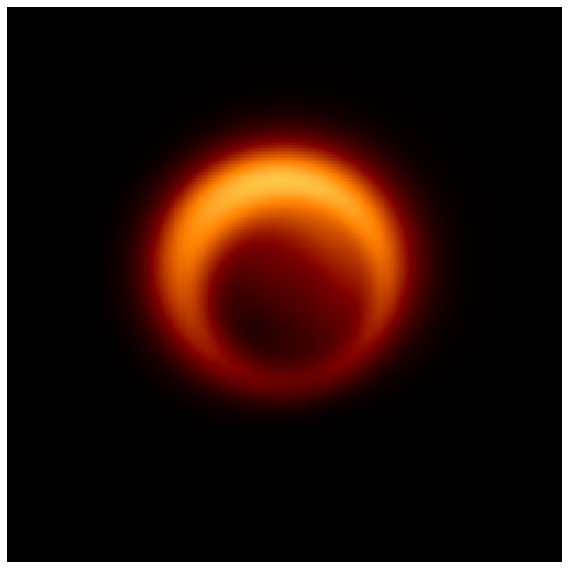
\includegraphics[height=.15\linewidth]{figures/starwarps_results/rotation30/gt/pavgimg_colorbar.pdf}} } \hspace{.55in} &
			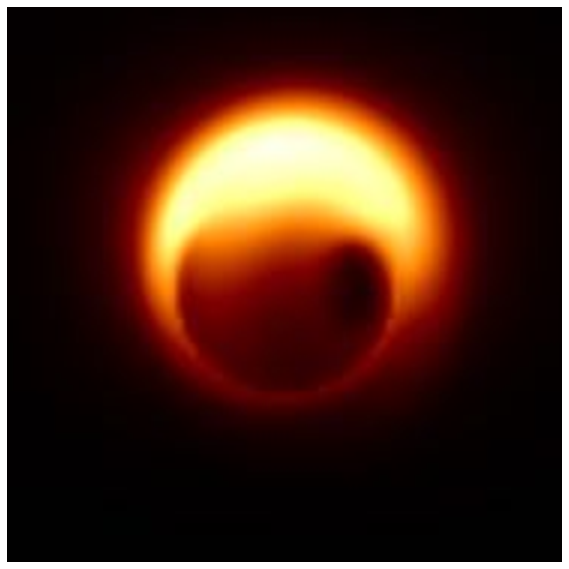
\includegraphics[height=.15\linewidth]{figures/starwarps_results/hotspot100sR2/gt/pavgimg_colorbar.pdf} \hspace{.55in} &
			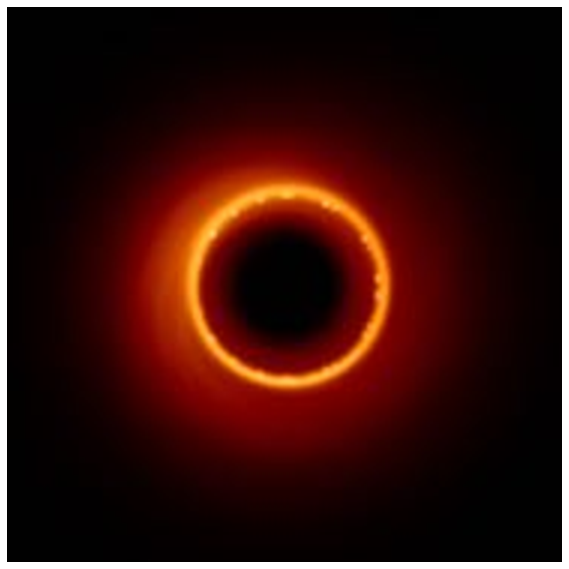
\includegraphics[height=.15\linewidth]{figures/starwarps_results/hotakamovie_02/gt/pavgimg_colorbar.pdf} \hspace{.55in} &
			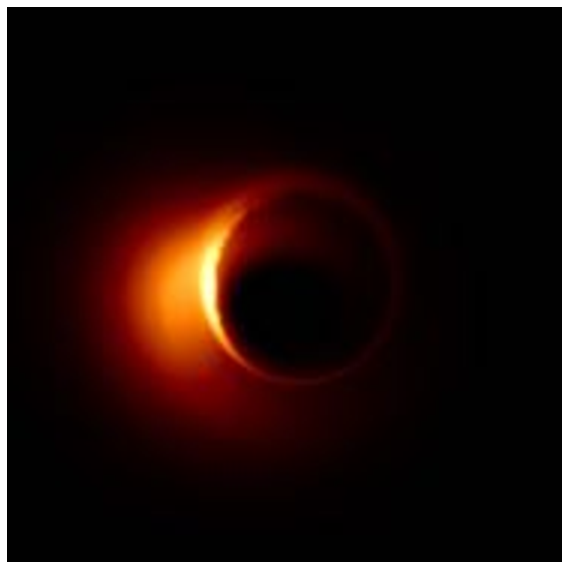
\includegraphics[height=.15\linewidth]{figures/starwarps_results/hotakamovie_45/gt/pavgimg_colorbar.pdf} \hspace{.55in}
			\\ \hline
			&\vspace{-.1in}&&&\\
			\multirow{1}{*}[0.9in]{ \rotatebox[origin=t]{90}{\small{\textsf{STD. DEVIATION}} }}
			& \hspace{0.01in}
			{{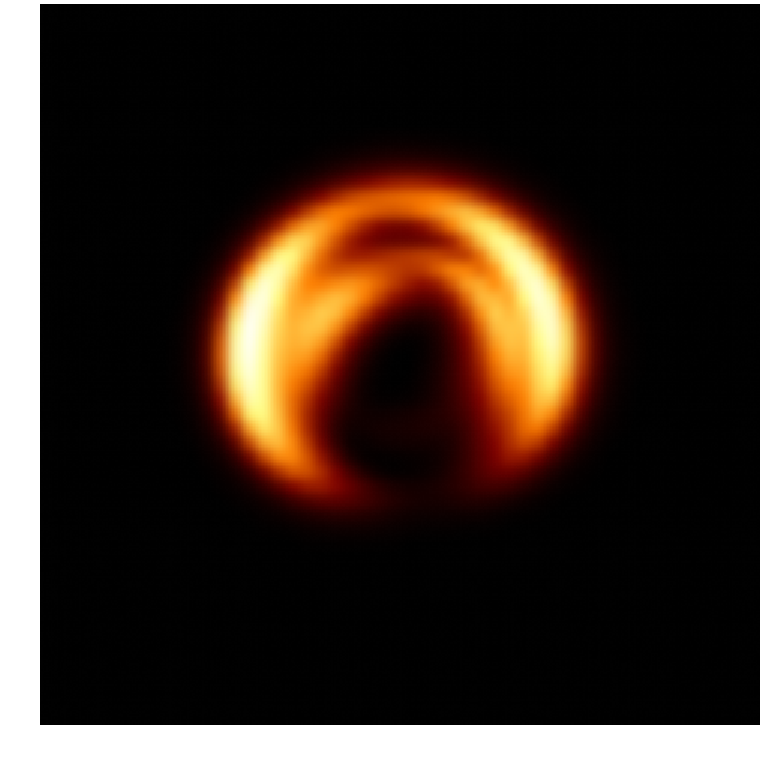
\includegraphics[height=.147\linewidth]{figures/starwarps_results/rotation30/gt/stdevimg_noaxis_r2.pdf}} } \hspace{.59in} & 
			
			\hspace{0.01in}
			 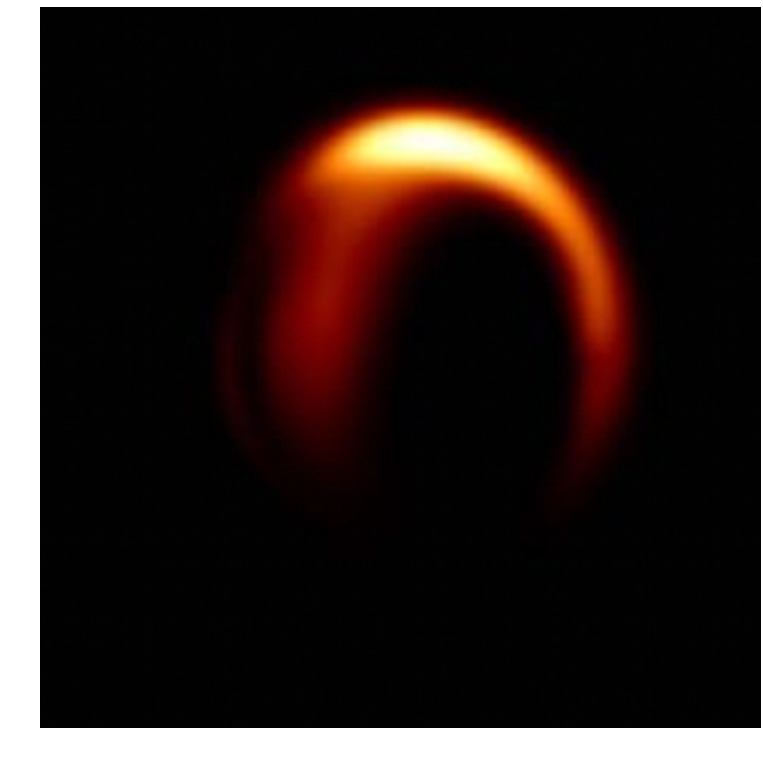
\includegraphics[height=.147\linewidth]{figures/starwarps_results/hotspot100sR2/gt/stdevimg_noaxis_r2.pdf}  \hspace{.59in} &
			
			\hspace{-0.01in} 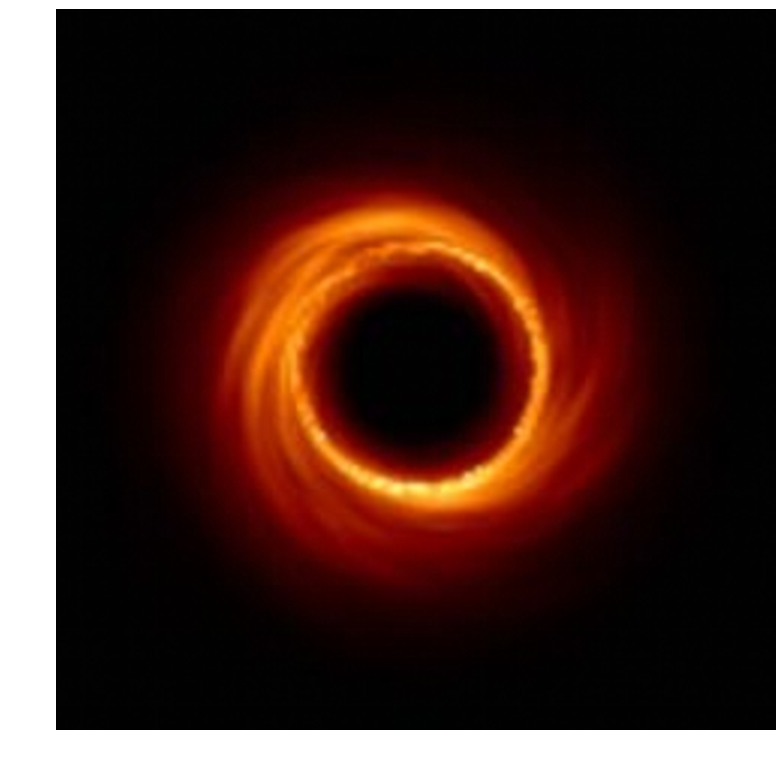
\includegraphics[height=.147\linewidth]{figures/starwarps_results/hotakamovie_02/gt/stdevimg_noaxis_r2.pdf}  \hspace{.55in} & 
			\hspace{-0.01in}
			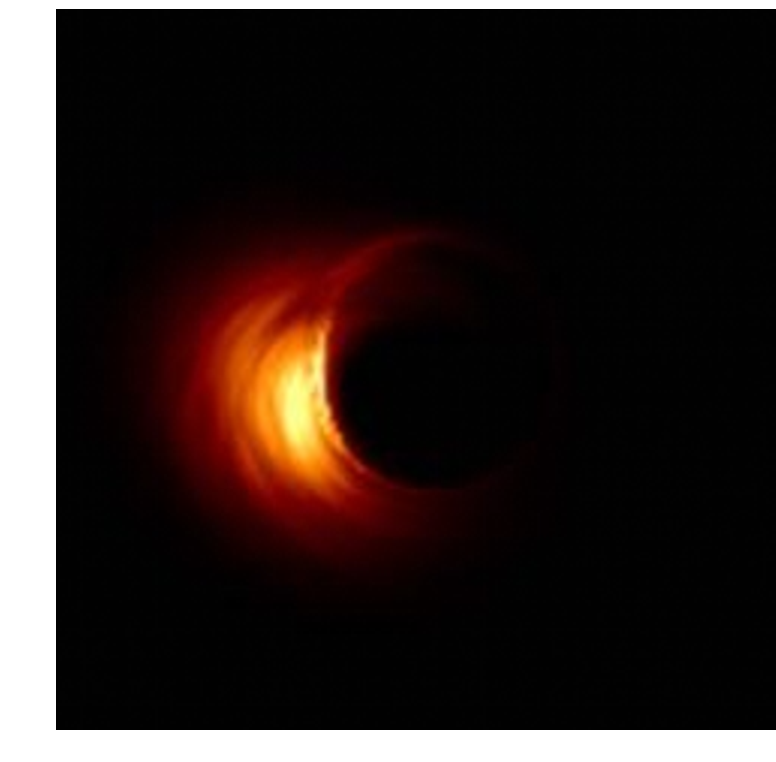
\includegraphics[height=.147\linewidth]{figures/starwarps_results/hotakamovie_45/gt/stdevimg_noaxis_r2.pdf} \hspace{.55in} 
			\\
		\end{tabular}
		\vspace{.1in}
		\caption{{\bf Ground truth videos:} The four ground truth sequences used to demonstrate results. We show a single frame from each sequence, the mean frame, and the spatial standard deviation of flux density. Video 1 consists of a $160 \mu$-arcsecond image~\cite{avery} that rotates $180^{\circ}$ over the course of a 12 hour observation (24 hour rotational period). Video 2 is a $120 \mu$-arcsecond view of an edge-on black hole disk with a rotating ``hot spot" predicted by~\cite{Broderick_Loeb_2006} with a rotational period of 2.78 hours. Video 3 and 4 are generated using a model of a black hole observed face on and at a $45^{\circ}$ inclination with a $160 \mu$-arcsecond field of view~\cite{Shiokawa_2013}. They assume a spin of 0.9375 with an Innermost Stable Circular Orbit (ISCO) rotational period of 8.96 minutes. The specified FOV and colormaps for the single frame and mean images are used for each corresponding video throughout the remainder of the paper. }
		%video 1: 1.2 max val
		%video 2: 1.6 maxval
		%video 3: .4 maxval
		%video 4: .8 maxval
		\label{fig:groundtruth}
	\end{center}
		\vspace{-.2in}
\end{figure*}

\vspace{-.07in}
\section{Dynamic Imaging Results}
\label{sec:results}

As data from the EHT 2017 campaign is yet to be released, in this section we demonstrate our method on synthetic EHT data and real data from the Very Long Baseline Array (VLBA). Additional results can be seen in the supplemental document and video. The StarWarps algorithm has been implemented as part of the publicly available python \texttt{eht-imaging}\footnote{\url{https://github.com/achael/eht-imaging}} library~\cite{andrew}.

\vspace{-.2in}
\subsection{Synthetic Data Generation} 

We demonstrate our algorithm on synthetic data generated from four different sequences of time-varying sources. These sequences include two realistic fluid simulations of a black hole accretion disk for different observing orientations~\cite{Shiokawa_2013}, a realistic sequence of a ``hot spot" rotating around a black hole~\cite{Broderick_Loeb_2006}, and a toy sequence evolving with pure rotation. The field of view of each sequence ranges from 120 to 160 $\mu$-arcseconds. A still frame from each sequence is shown in Figure~\ref{fig:groundtruth}. To help give a sense of the variation in each sequence, the figure also displays the mean and standard deviation of flux density. We refer to these sequences by their video number, indicated in the figure. 



In order to demonstrate the quality of results under various observing conditions, VLBI observations of SgrA* at 1.3 mm (230 GHz) are simulated assuming
 three different telescope arrays.  The first array, EHT2017, consists of the 8 telescopes at 6 distinct locations that were used to collect measurements for the Event Horizon Telescope in the spring of 2017. The uv-coverage for this array can be seen in Figure~\ref{fig:staticimaging}. The second array, EHT2017+, augments the EHT2017 array with 3 potential additions to the EHT: Plateau de Bure (PDB), Haystack (HAY), and Kitt Peak (KP) Observatory. 
Details on telescopes used in the EHT2017 and EHT2017+ array are shown in Table~\ref{tab:telescopes}.  
The third array, FUTURE, consists of 9 additional telescopes. The uv-coverage of these latter two arrays, along with a colorbar indicating the time of each measurement, is shown in Figures~\ref{fig:uvcov2}. 
%Details on telescopes used in these arrays are shown in the supplemental material.


Visibility measurements are generated using the python \texttt{eht-imaging} library~\cite{andrew}. %assuming a 4 GHz bandwidth with a 100 second integration time. 
Realistic thermal noise, resulting from a bandwidth ($\Delta \nu$) of 4 GHz and a 100 second integration time ($t_{\rm int}$), is introduced on each visibility. The standard deviation of thermal noise is given by
\begin{align}
\sigma = \frac{1}{0.88} \sqrt{\frac{\mbox{SEFD}_1 \times \mbox{SEFD}_2 }{2 \times \Delta \nu \times t_{\rm int} } },
\label{eq:thermal}
\end{align}

\noindent{for System Equivalent Flux Density (SEFD) of the two telescopes corresponding to each visibility\footnote{The factor of 1/0.88 is due to information loss due to recording 2-bit quantized data-streams at each telescope~\cite{TMS}.}~\cite{taylor1999synthesis}.  %, and using bandwidth $\Delta \nu$ and integration time $t_{int}$.}
% in the absense of atmospheric error
%Atmospheric phase error is also introduced into measurements using the \texttt{eht-imaging} library. 
Random station-based atmospheric phases drawn from a uniform distribution at each time step are introduced into measurements using the \texttt{eht-imaging} library. 
In Videos 2-4 a set of measurements is sampled every 5 minutes over a roughly 14 hour duration, resulting in 173 time steps. In Video 1 only 30 time steps are measured over a 12 hour duration. 
}


\begin{figure}[h!]
	\centering
	%{\includegraphics[height=.28\linewidth]{figures/uvcoverage/uv_eht2017.pdf}}
	{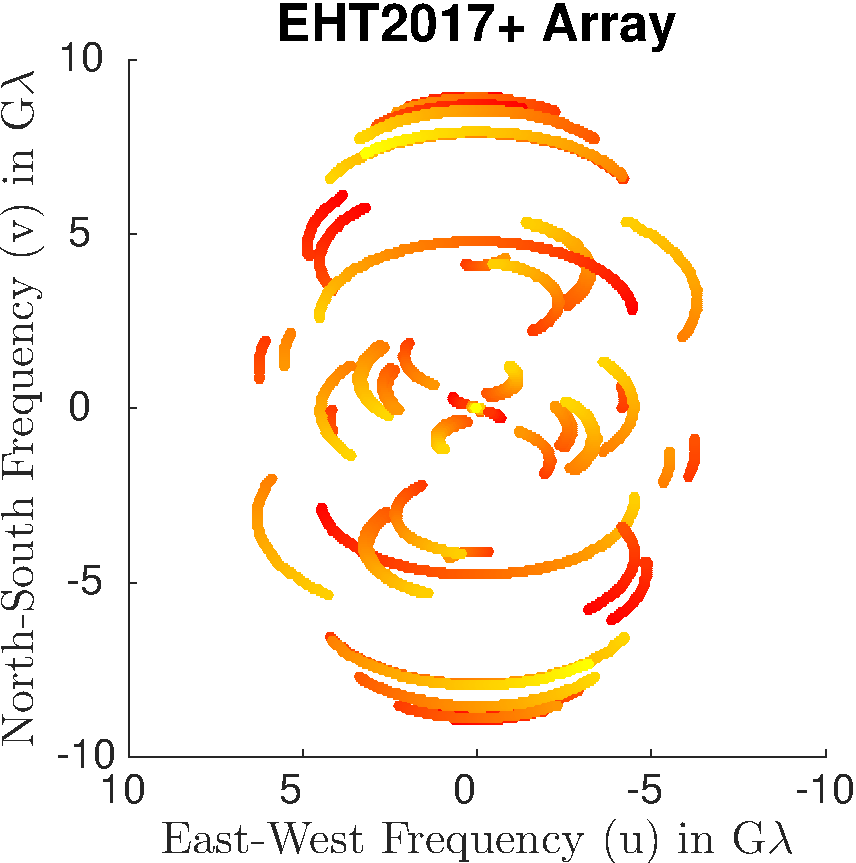
\includegraphics[height=.38\linewidth]{figures/uvcoverage/uv_ehtfuture2_2.pdf}}
	{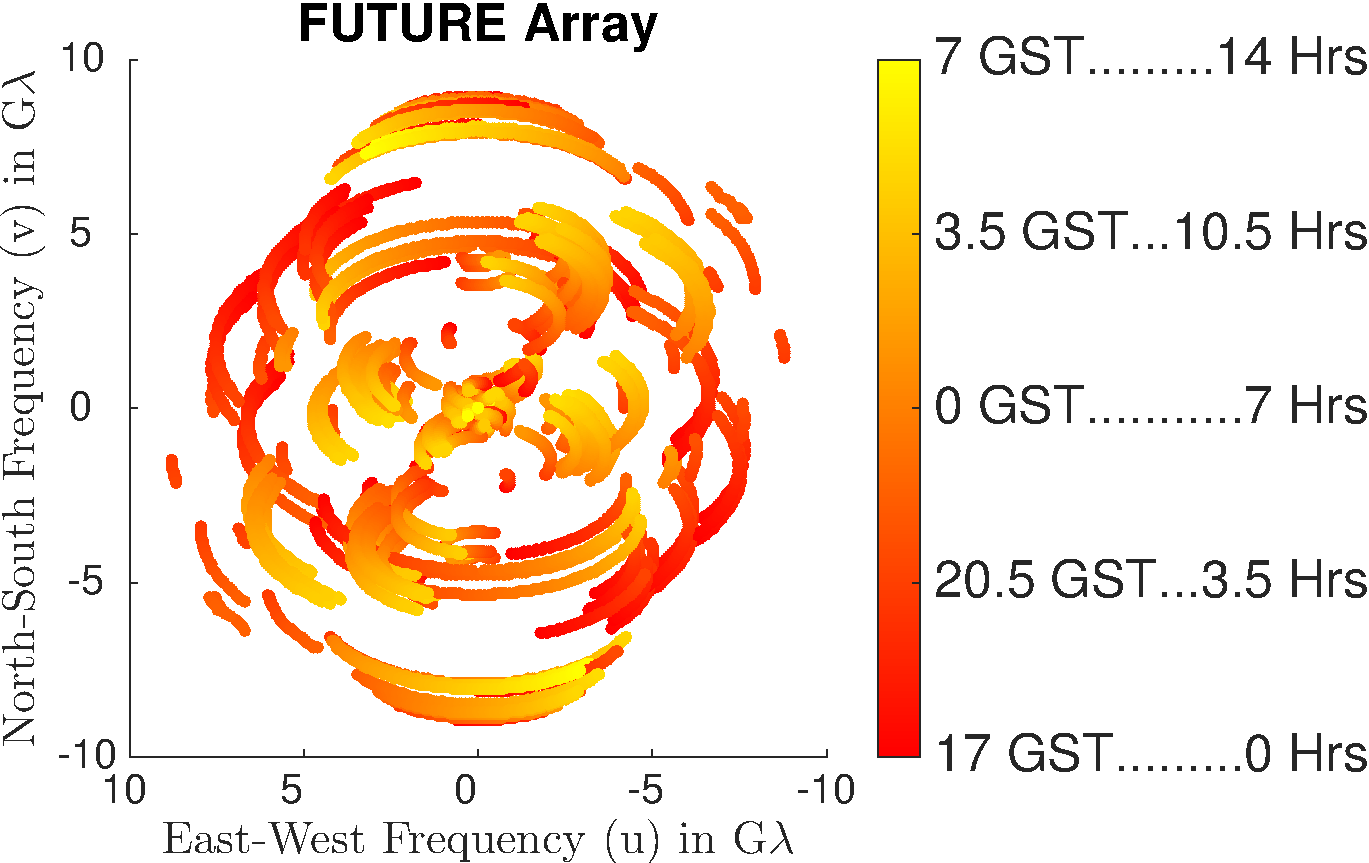
\includegraphics[height=.38\linewidth]{figures/uvcoverage/uv_ehtfuture1_2.pdf}}
	\caption{{\bf Time-varying uv-coverage:} The uv-coverage for EHT2017+ and FUTURE arrays when observing SgrA∗. The uv-coverage for the EHT2017 array can be seen in Figure~\ref{fig:staticimaging}. 
		Baselines are colored by the time of each observation relative to the start time, indicated by the colorbar to the right.}
	\label{fig:uvcov2}

\end{figure}


\begin{table}[!t]
	\begin{center}
		\caption{EHT 2017 Station Parameters}
		\label{tab::eht_station}
		\begin{tabular}{ccc}
 Telescope & Location & SEFD (Jy) \\ \hline
 ALMA & Chile & 110 \\ 
 APEX & Chile & 22000 \\ 
 LMT & Mexico & 560 \\
 SMT & Arizona & 11900 \\ 
 SMA & Hawaii & 4900 \\
 JCMT & Hawaii & 4700 \\ 
 PV & Spain & 2900 \\ 
 SPT & South Pole & 1600 \\ \hline
 PDB* & France & 1600 \\ 
 HAY* & Massachusetts & 2500 \\ 
 KP* & Arizona & 2500 \\ \hline
		\end{tabular}\\
	\end{center}
	\bigskip
	\footnotesize{The location and SEFD of each telescope in the EHT2017 and EHT2017+ arrays. These parameters and locations were used to generate the uv-trajectories in frequency space shown in Figure~\ref{fig:staticimaging} and~\ref{fig:uvcov2}. Telescope names followed by a star (*) were not included in the EHT2017 array.}
	\label{tab:telescopes}
	\vspace{-0.3in}
\end{table}



%\begin{table}[h!]
%\begin{center}
%\begin{tabular}{ c c c }
% Telescope & Location & SEFD (Jy) \\ \hline
% ALMA & Chile & 110 \\ 
% APEX & Chile & 22000 \\ 
% LMT & Mexico & 560 \\
% SMT & Arizona & 11900 \\ 
%SMA & Hawaii & 4900 \\
%JCMT & Hawaii & 4700 \\ 
% PV & Spain & 2900 \\ 
% SPT & South Pole & 1600 \\ \hline
% PDB* & France & 1600 \\ 
% HAY* & Massachusetts & 2500 \\ 
%  KP* & Arizona & 2500 \\ \hline
%\end{tabular}
%\end{center}
%\caption{ The location and SEFD of each telescope in the EHT2017 and EHT2017+ arrays. These parameters and locations were used to generate the uv-trajectories in frequency space shown in Figure~\ref{fig:staticimaging} and~\ref{fig:uvcov2}. Telescope names followed by a star (*) were not included in the EHT2017 array. }
%\label{tab:telescopes}
%\vspace{-0.3in}
%\end{table}

\vspace{-.1in}
\subsection{Static Evolution Model (No Warp)}
\label{sec:nomotionresults}

We first demonstrate results of our method under a static evolution model. In this case, we fix parameters $\theta$ such that $A=\mathds{1}$. This assumes that there is no global motion under a persistent warp field, but only perturbations around a fairly static scene. Despite this incorrect assumption (especially in Videos 1 and 2), this simple model results in reconstructions that surpass the state-of-the-art methods, and recovers distinctive structures that appear in the underlying source images. 


\subsubsection{Synthetic Data Result Comparison}

\begin{figure*}
	\begin{center}
		\vspace{-0.5in}
		%\hspace*{-2.3cm}
		\setlength{\tabcolsep}{3pt}
		
		\hspace{-0.5in}\normalsize{\textsf{BLURRED TRUE MEAN}}  \hspace{5.5cm} \normalsize{\textsf{NORMALIZED RMSE}} 
		\vspace{0.1in}
		
		
%	\begin{tabular}{ c " c}
%		VIDEO 1& VIDEO 2 \\ \thickhline
%		& \vspace{-.1in} \\
%		VIDEO 3 & VIDEO 4
%	\end{tabular}
%	\qquad
%		\begin{tabular}{ c " c}
%		{{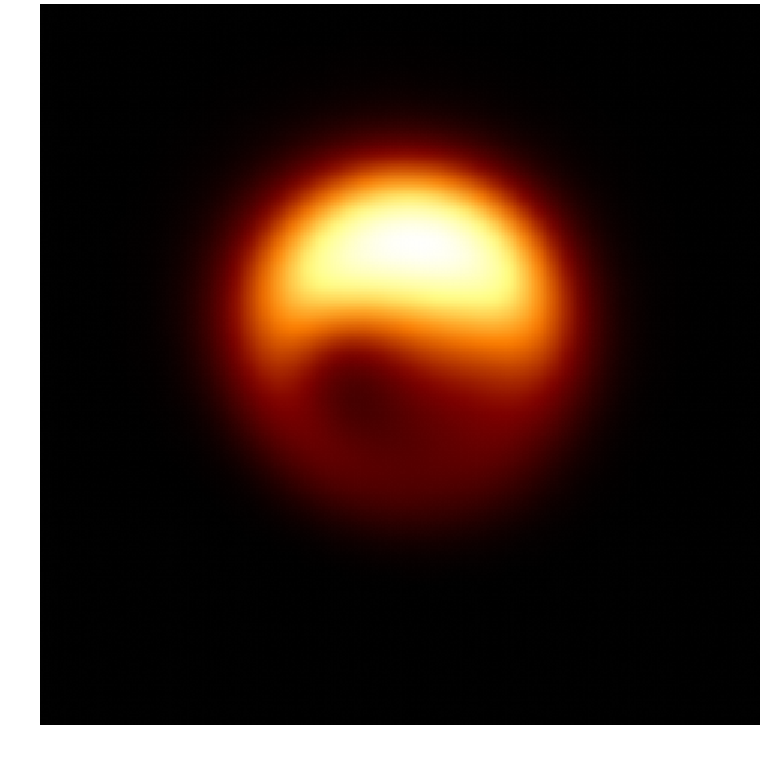
\includegraphics[height=.1\linewidth]{figures/starwarps_results/rotation30/gt/frames/gt_15_blurredbeam75_noaxis.pdf}} } & {{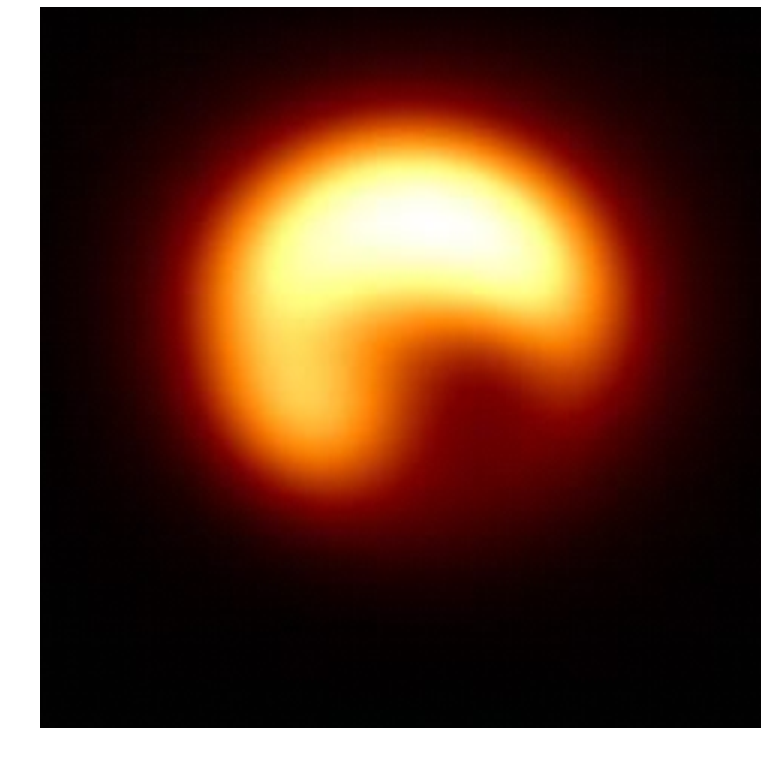
\includegraphics[height=.1\linewidth]{figures/starwarps_results/hotspot100sR2/gt/frames/gt_115_blurredbeam75_noaxis.pdf}} } \\ \thickhline
%		& \vspace{-.1in} \\
%	{{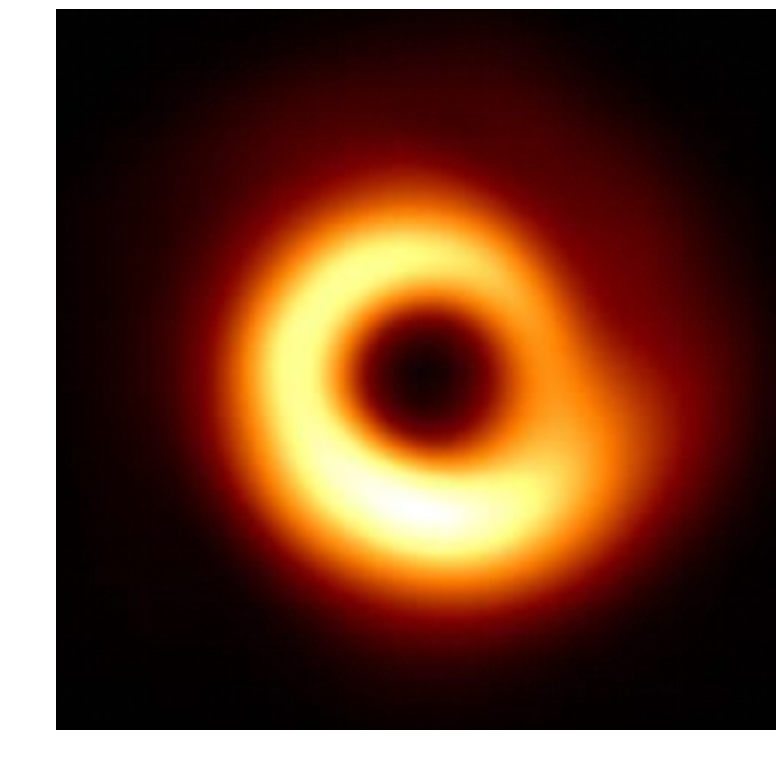
\includegraphics[height=.1\linewidth]{figures/starwarps_results/hotakamovie_02/gt/frames/gt_85_blurredbeam75_noaxis.pdf}} } & {{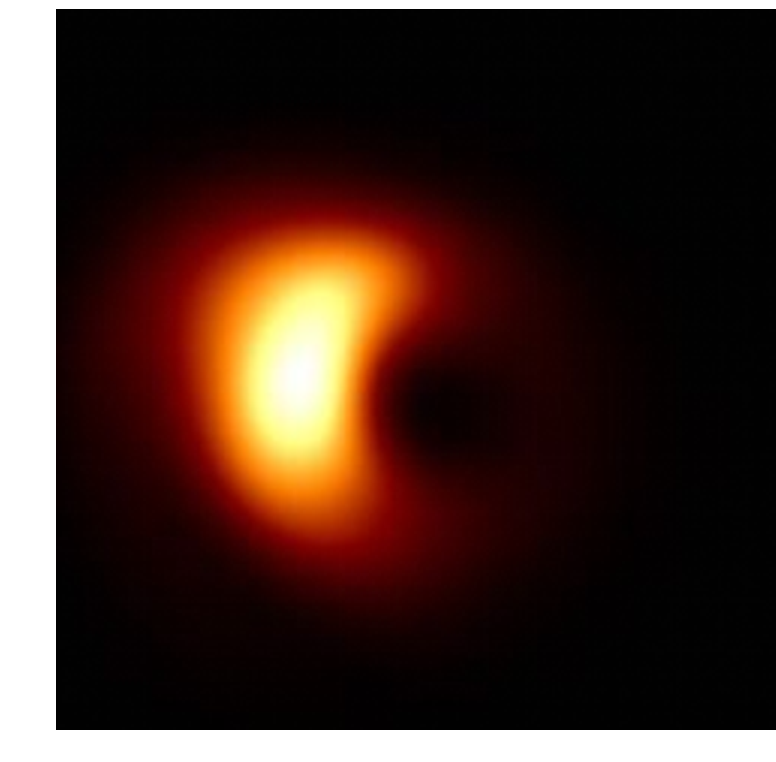
\includegraphics[height=.1\linewidth]{figures/starwarps_results/hotakamovie_45/gt/frames/gt_63_blurredbeam75_noaxis.pdf}} }
%		\end{tabular}
						\begin{tabular}{ c " c}
							\hspace{-.06in} \textsf{Video 1} & \hspace{-.06in} \textsf{Video 2} \\
							{{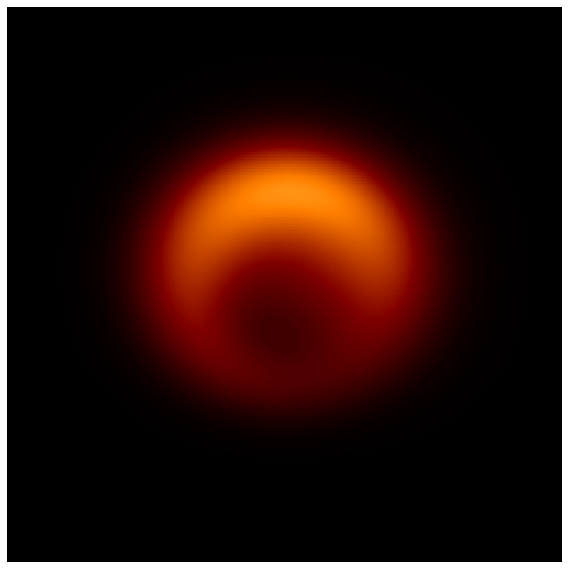
\includegraphics[height=.1\linewidth]{figures/starwarps_results/rotation30/gt/pavgImg_blurredbeam75_noaxis.pdf}} } & {{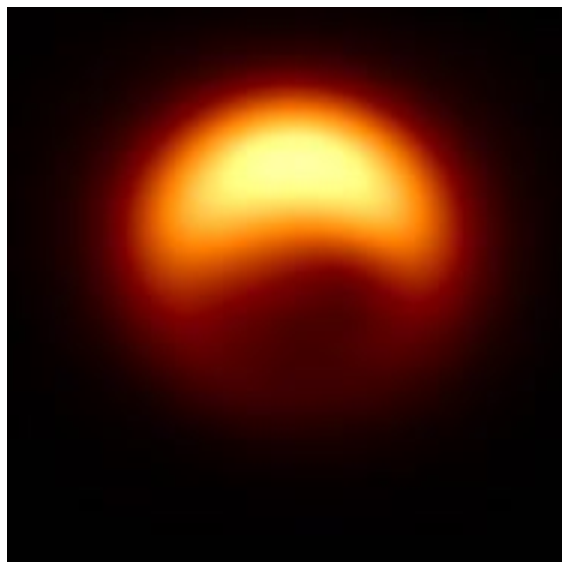
\includegraphics[height=.1\linewidth]{figures/starwarps_results/hotspot100sR2/gt/pavgImg_blurredbeam75_noaxis.pdf}} } \\ \thickhline
							& \vspace{-.1in} \\
							\hspace{-.06in} \textsf{Video 3} & \hspace{-.06in} \textsf{Video 4} \\
							{{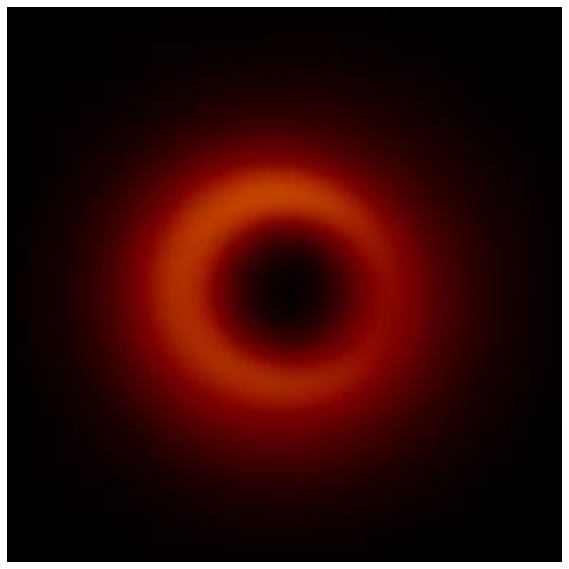
\includegraphics[height=.1\linewidth]{figures/starwarps_results/hotakamovie_02/gt/pavgImg_blurredbeam75_noaxis.pdf}} } & {{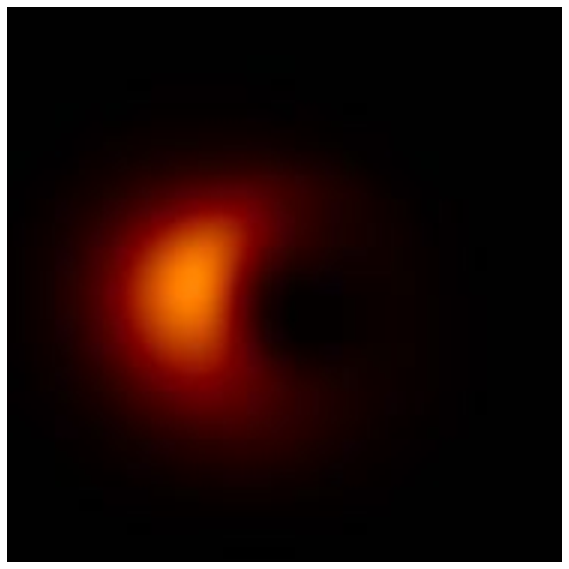
\includegraphics[height=.1\linewidth]{figures/starwarps_results/hotakamovie_45/gt/pavgImg_blurredbeam75_noaxis.pdf}} }
						\end{tabular}	
	%	\qquad	
		\qquad
		\begin{tabular}{ r | c | c | c | c " c | c | c | c}
			& \rotatebox[origin=t]{90}{\small{\textsf{EHT 2017}} } \rotatebox[origin=t]{90}{\small{\textsf{NO ATM.}} }  & \rotatebox[origin=t]{90}{\small{\textsf{EHT 2017}} } \rotatebox[origin=t]{90}{\small{\textsf{ATM.}} } & \rotatebox[origin=t]{90}{\small{\textsf{EHT 2017+}} } \rotatebox[origin=t]{90}{\small{\textsf{ATM.}} } &\rotatebox[origin=t]{90}{\small{\textsf{FUTURE}} } \rotatebox[origin=t]{90}{\small{\textsf{ATM.}} } & \rotatebox[origin=t]{90}{\small{\textsf{EHT 2017}} } \rotatebox[origin=t]{90}{\small{\textsf{NO ATM.}} }  & \rotatebox[origin=t]{90}{\small{\textsf{EHT 2017}} } \rotatebox[origin=t]{90}{\small{\textsf{ATM.}} } & \rotatebox[origin=t]{90}{\small{\textsf{EHT 2017+}} } \rotatebox[origin=t]{90}{\small{\textsf{ATM.}} } &\rotatebox[origin=t]{90}{\small{\textsf{FUTURE}} } \rotatebox[origin=t]{90}{\small{\textsf{ATM.}} }  \\ \hline
			{\small{\textsf{StarWarps Mean} } } & {\bf {0.67} }& {\bf {0.65}} & {\bf {0.55} }&  {\bf {0.55}}& {\bf {0.74}} & {\bf {0.73} }& {\bf {0.73}} &  0.71 \\ 
				\cite{freek} & 1.05  & 0.82 & 0.73  & 0.68 &  0.98 & 1.21 & 0.99 & 0.35 \\ 
				\cite{andrew} & 0.79 & 0.80 & 0.73 & 0.63 & 0.83& 1.05 & 0.81 & {\bf 0.23}  \\  \thickhline
				\small{\textsf{StarWarps Mean} } & {\bf 0.32} & {\bf 0.55} & 0.67 & {\bf 0.36} & {\bf 0.34} & {\bf 0.44} & {\bf 0.23} & {\bf 0.31} \\
				\cite{freek} & 0.93 & 0.90 & {\bf 0.53} & 0.51 & 0.84 & 0.75 & 1.02 & 0.61 \\
				\cite{andrew} &0.84 & 0.85 & 0.71 &  0.39  & 0.60 & 0.50 & 0.60 & 0.47
			\end{tabular}

		\vspace{0.4in}
		
		\hspace*{-1.3cm}
		\begin{tabular}{  c c | c  c  c  c "  c  c  c  c  }
			%\hline
			& \small{\textsf{Array:}} &\small{\textsf{EHT 2017}}   &\small{\textsf{EHT 2017 }} &\small{\textsf{EHT2017+}}    &\small{\textsf{FUTURE}}    &\small{\textsf{EHT 2017}}   &\small{\textsf{EHT 2017 }} &\small{\textsf{EHT2017+}}    &\small{\textsf{FUTURE}}     \\ 
			&\vspace{-.1in} & & & & & & & &\\
			& \small{\textsf{Error:}} &\small{\textsf{NO ATM.}}   &\small{\textsf{ATM.}} &\small{\textsf{ATM.}}    &\small{\textsf{ATM.}}  &\small{\textsf{NO ATM.}}   &\small{\textsf{ATM.}} &\small{\textsf{ATM.}}    &\small{\textsf{ATM.}}   \\ \hline
%			&\vspace{-.1in} & & & & & & & &\\
%			\multirow{2}{*}[0.2in]{ \rotatebox[origin=t]{90}{\small{\textsf{StarWarps}} }}   \hspace{-0.3in} & \multirow{1}{*}[0.5in]{ \rotatebox[origin=t]{90}{\small{\textsf{FRAME}} }}
%			&
%			{{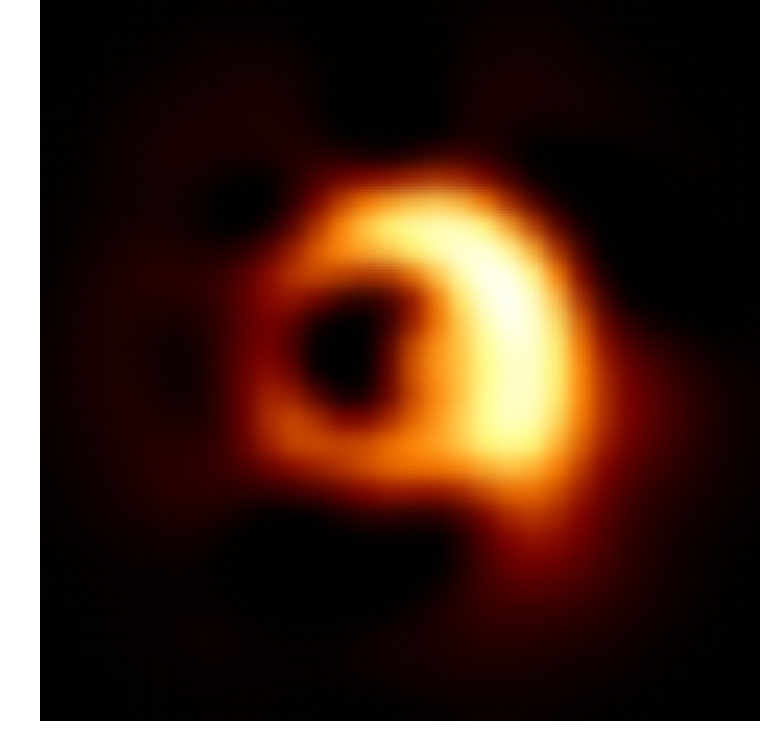
\includegraphics[height=.1\linewidth]{figures/starwarps_results/rotation30/eht2017_100_visibility/nomotion/frames/mean_noaxis_15.pdf}} } &
%			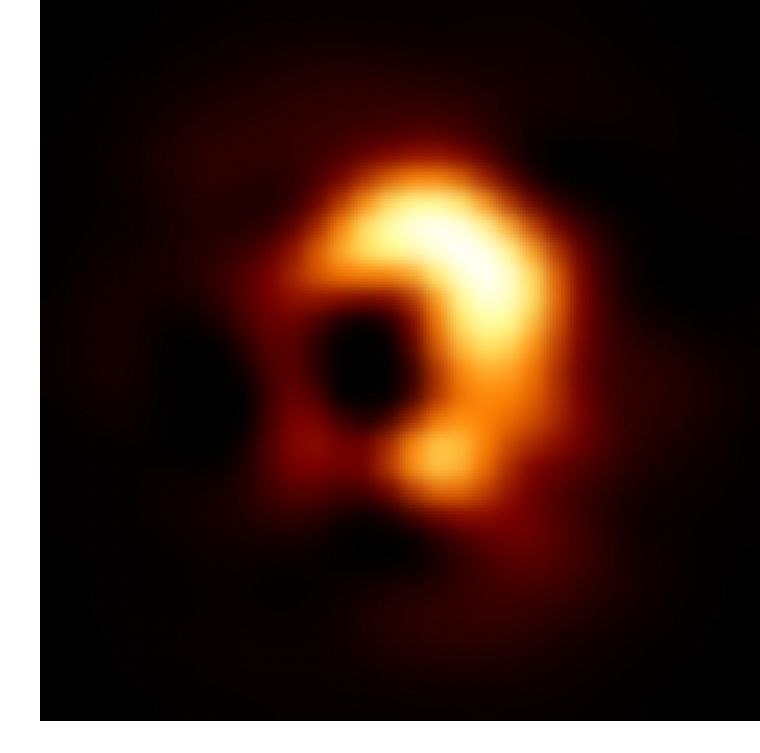
\includegraphics[height=.1\linewidth]{figures/starwarps_results/rotation30/eht2017_100_amp-bispectrum/nomotion/frames/mean_noaxis_15.pdf} &
%			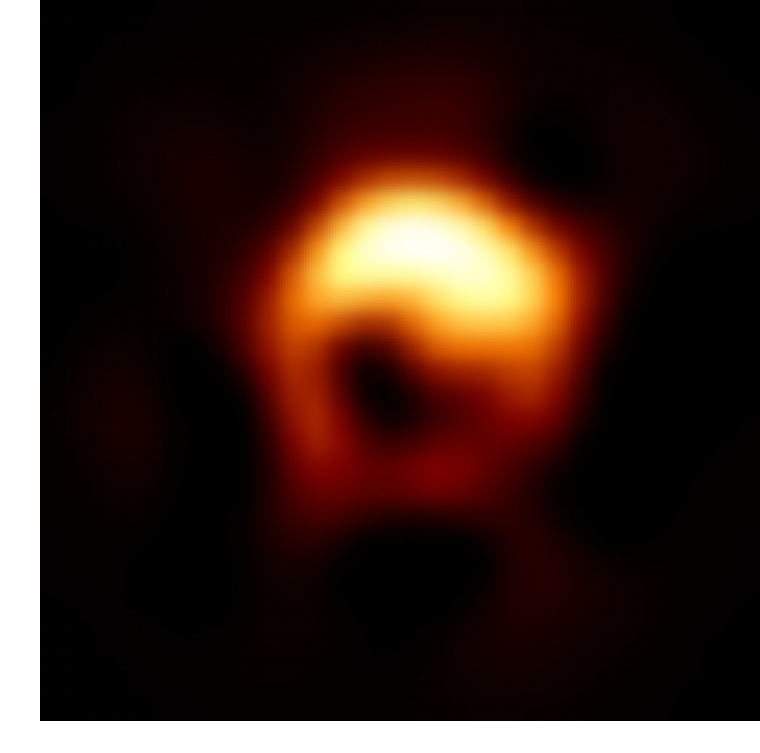
\includegraphics[height=.1\linewidth]{figures/starwarps_results/rotation30/ehtfuture2_100_amp-bispectrum/nomotion/frames/mean_noaxis_15.pdf} &
%			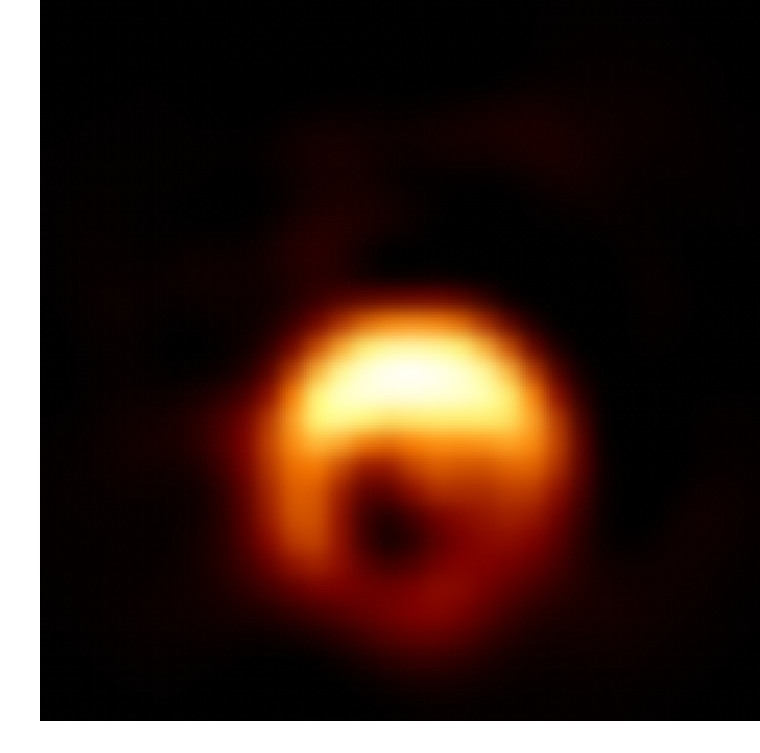
\includegraphics[height=.1\linewidth]{figures/starwarps_results/rotation30/ehtfuture1_100_amp-bispectrum/nomotion/frames/mean_noaxis_15.pdf}  
%			&
%			{{\includegraphics[height=.1\linewidth]{figures/starwarps_results/hotspot100sR2/eht2017_100_visibility/nomotion/frames/mean_noaxis_115.pdf}} } &
%			\includegraphics[height=.1\linewidth]{figures/starwarps_results/hotspot100sR2/eht2017_100_amp-bispectrum/nomotion/frames/mean_noaxis_115.pdf} &
%			\includegraphics[height=.1\linewidth]{figures/starwarps_results/hotspot100sR2/ehtfuture2_100_amp-bispectrum/nomotion/frames/mean_noaxis_115.pdf} &
%			\includegraphics[height=.1\linewidth]{figures/starwarps_results/hotspot100sR2/ehtfuture1_100_amp-bispectrum/nomotion/frames/mean_noaxis_115.pdf} \\
			&\vspace{-.1in} & & & & & & & &\\
			 \multirow{2}{*}[0.6in]{ \rotatebox[origin=t]{90}{\small{\textsf{StarWarps}} }}   \hspace{-0.3in} &	\multirow{1}{*}[0.45in]{ \rotatebox[origin=t]{90}{\small{\textsf{Mean}} }}
			&
			{{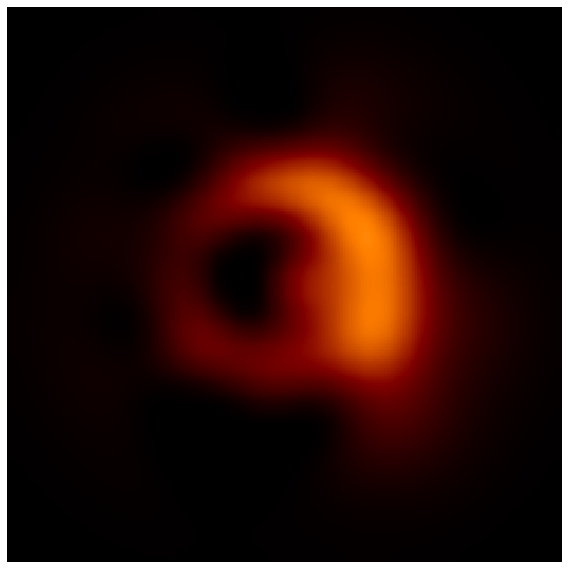
\includegraphics[height=.1\linewidth]{figures/starwarps_results/rotation30/eht2017_100_visibility/nomotion/pavgimg_noaxis.pdf}} } &
			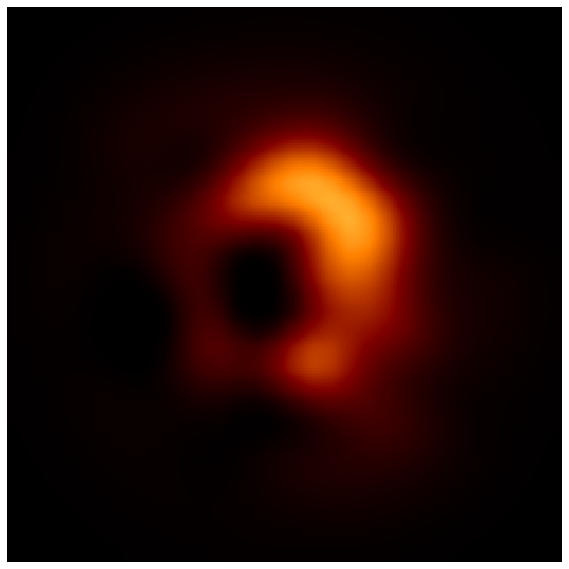
\includegraphics[height=.1\linewidth]{figures/starwarps_results/rotation30/eht2017_100_amp-bispectrum/nomotion/pavgimg_noaxis.pdf} &
			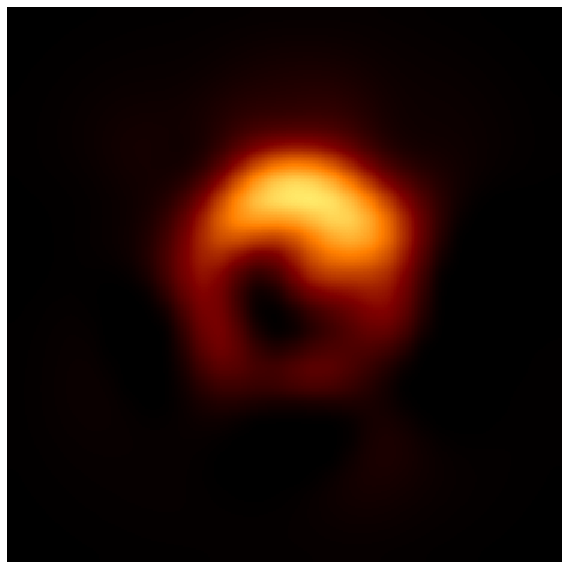
\includegraphics[height=.1\linewidth]{figures/starwarps_results/rotation30/ehtfuture2_100_amp-bispectrum/nomotion/pavgimg_noaxis.pdf} &
			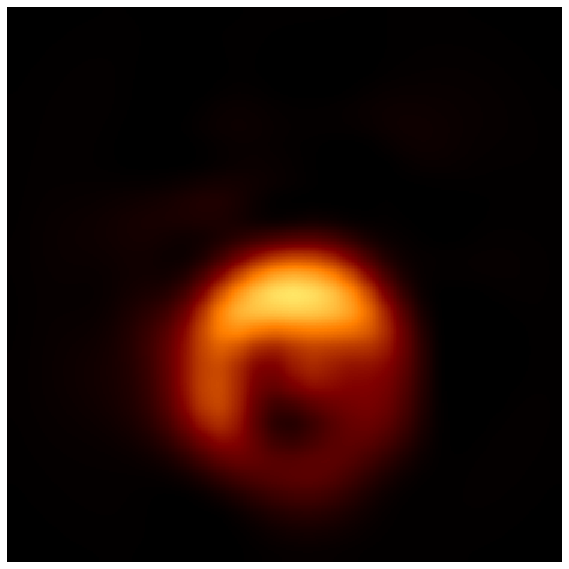
\includegraphics[height=.1\linewidth]{figures/starwarps_results/rotation30/ehtfuture1_100_amp-bispectrum/nomotion/pavgimg_noaxis.pdf} 
			&
			{{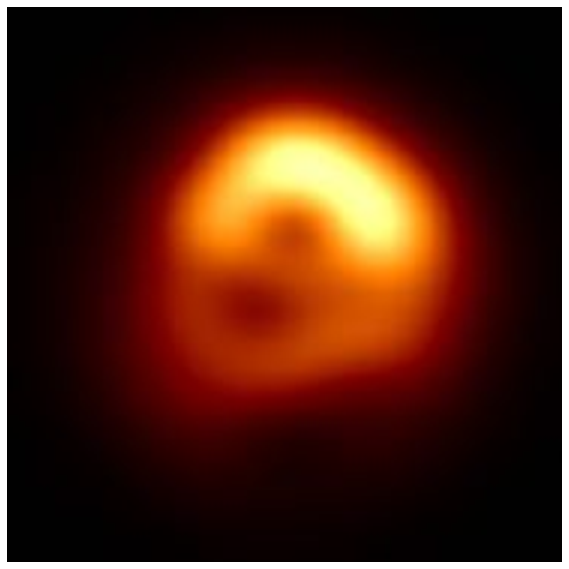
\includegraphics[height=.1\linewidth]{figures/starwarps_results/hotspot100sR2/eht2017_100_visibility/nomotion/pavgimg_noaxis.pdf}} } &
			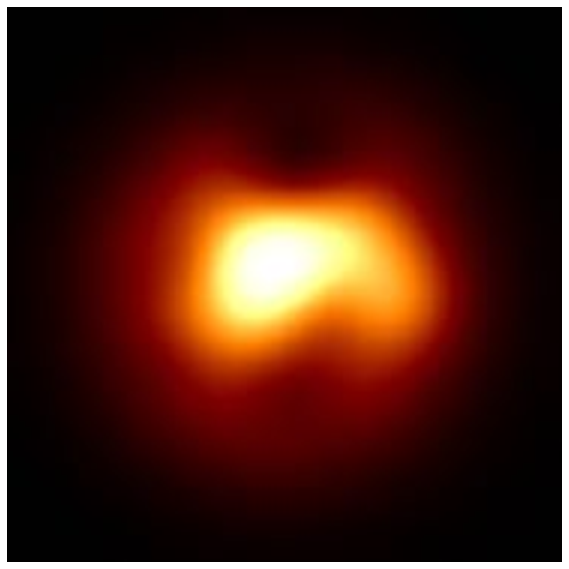
\includegraphics[height=.1\linewidth]{figures/starwarps_results/hotspot100sR2/eht2017_100_amp-bispectrum/nomotion/pavgimg_noaxis.pdf} &
			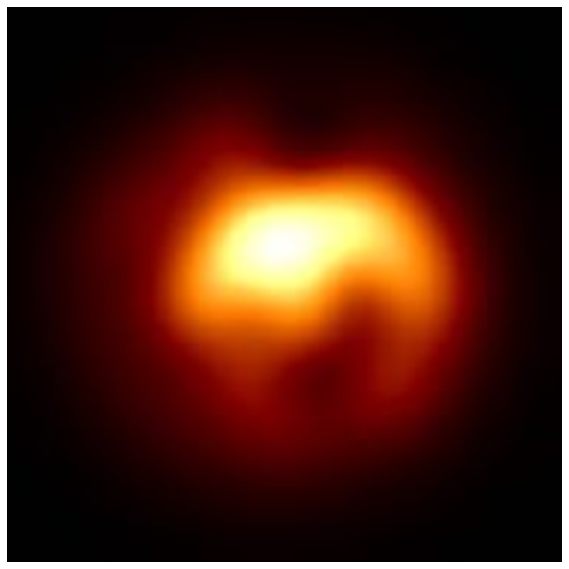
\includegraphics[height=.1\linewidth]{figures/starwarps_results/hotspot100sR2/ehtfuture2_100_amp-bispectrum/nomotion/pavgimg_noaxis.pdf} &
			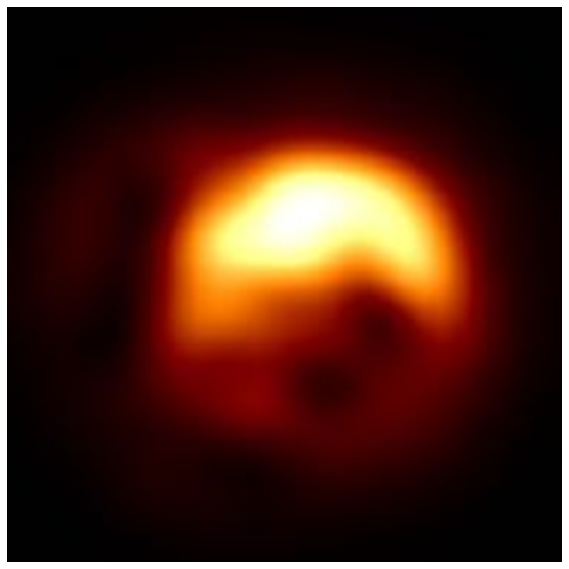
\includegraphics[height=.1\linewidth]{figures/starwarps_results/hotspot100sR2/ehtfuture1_100_amp-bispectrum/nomotion/pavgimg_noaxis.pdf} 
			\\   \hline
			&\vspace{-.1in} & & & & & & & &\\
			\multirow{2}{*}[0.6in]{ \rotatebox[origin=t]{90}{\small{\textsf{MEM \& TV Regularization}} }}  \hspace{-0.3in} & \multirow{1}{*}[0.4in]{ \rotatebox[origin=t]{90}{\small{\textsf{\cite{freek}}} }}
			&
			{{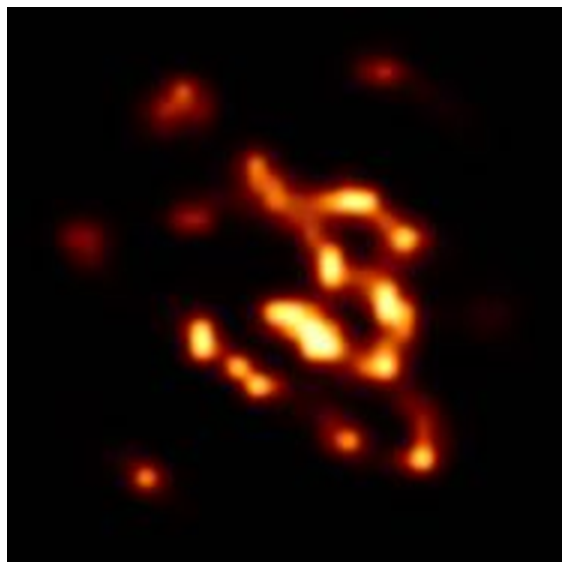
\includegraphics[height=.1\linewidth]{figures/freeksmoothingresults/im_vis_rotation30_tint100_eht2017_directim_maxit100_it0.pdf}} } &
			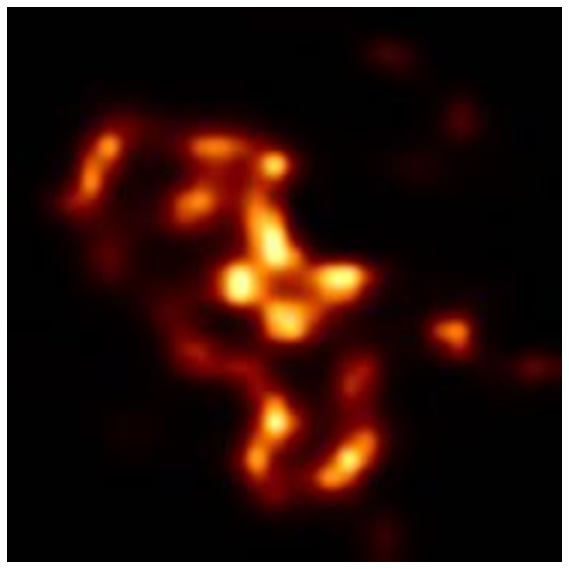
\includegraphics[height=.1\linewidth]{figures/freeksmoothingresults/im_apar_rotation30_tint100_eht2017_directim_maxit100_it0.pdf} &
			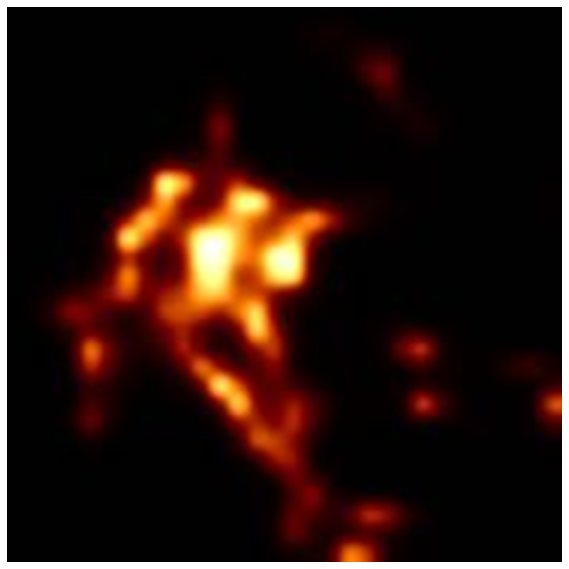
\includegraphics[height=.1\linewidth]{figures/freeksmoothingresults/im_apar_rotation30_tint100_ehtfuture2_directim_maxit100_it0.pdf} &
			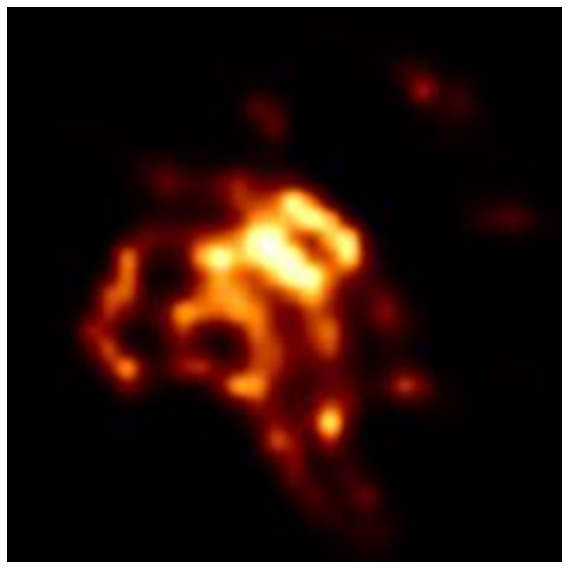
\includegraphics[height=.1\linewidth]{figures/freeksmoothingresults/im_apar_rotation30_tint100_ehtfuture1_directim_maxit100_it0.pdf} 
			&
			{{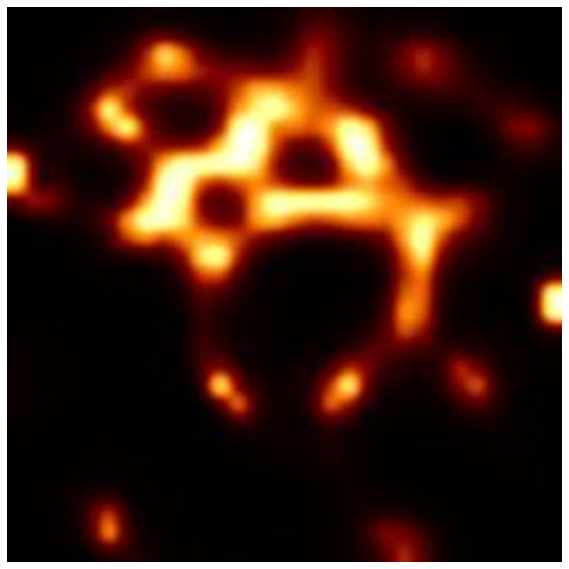
\includegraphics[height=.1\linewidth]{figures/freeksmoothingresults/im_vis_hotspot100sR2_tint100_eht2017_directim_maxit100_it0.pdf}} } &
			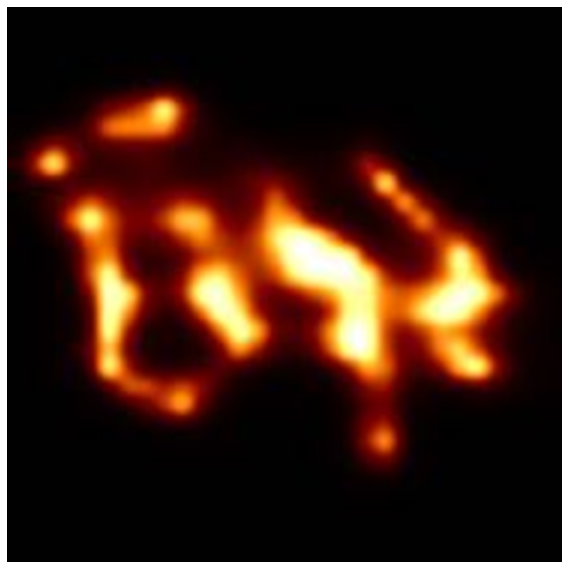
\includegraphics[height=.1\linewidth]{figures/freeksmoothingresults/im_apar_hotspot100sR2_tint100_eht2017_directim_maxit100_it0.pdf} &
			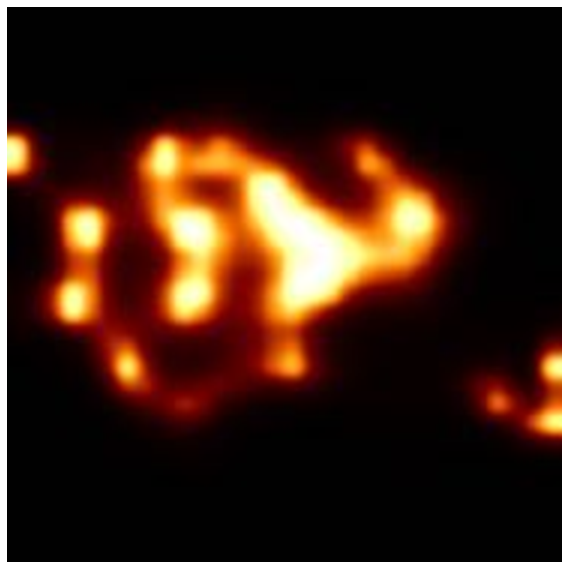
\includegraphics[height=.1\linewidth]{figures/freeksmoothingresults/im_apar_hotspot100sR2_tint100_ehtfuture2_directim_maxit100_it0.pdf} &
			\includegraphics[height=.1\linewidth]{figures/freeksmoothingresults/im_apar_hotspot100sR2_tint100_ehtfuture1_directim_maxit100_it0.pdf} 
			\\
			&\vspace{-.1in} & & & & & & & &\\
			&	\multirow{1}{*}[0.4in]{ \rotatebox[origin=t]{90}{\small{\textsf{\cite{andrew}}} }}
			&
			{{\includegraphics[height=.1\linewidth]{figures/starwarps_results/rotation30/eht2017_100_compare/none_vis_blur025.pdf}} } &
			\includegraphics[height=.1\linewidth]{figures/starwarps_results/rotation30/eht2017_100_compare/none_amp-clphase_blur025.pdf} &
			\includegraphics[height=.1\linewidth]{figures/starwarps_results/rotation30/ehtfuture2_100_compare/none_amp-clphase_blur025.pdf} &
			\includegraphics[height=.1\linewidth]{figures/starwarps_results/rotation30/ehtfuture1_100_compare/none_amp-clphase_blur025.pdf} 
			&
			{{\includegraphics[height=.1\linewidth]{figures/starwarps_results/hotspot100sR2/eht2017_100_compare/none_vis_blur025.pdf}} } &
			\includegraphics[height=.1\linewidth]{figures/starwarps_results/hotspot100sR2/eht2017_100_compare/none_amp-clphase_blur025.pdf} &
			\includegraphics[height=.1\linewidth]{figures/starwarps_results/hotspot100sR2/ehtfuture2_100_compare/none_amp-clphase_blur025.pdf} &
			\includegraphics[height=.1\linewidth]{figures/starwarps_results/hotspot100sR2/ehtfuture1_100_compare/none_amp-clphase_blur025.pdf} 
			\\   \thickhline
			
%			&\vspace{-.1in} & & & & & & & &\\
%			\multirow{2}{*}[0.2in]{ \rotatebox[origin=t]{90}{\small{\textsf{StarWarps}} }}  \hspace{-0.3in} & \multirow{1}{*}[0.5in]{ \rotatebox[origin=t]{90}{\small{\textsf{FRAME}} }}
%			&
%			{{\includegraphics[height=.1\linewidth]{figures/starwarps_results/hotakamovie_02/eht2017_100_visibility/nomotion/frames/mean_noaxis_85.pdf}} } &
%			\includegraphics[height=.1\linewidth]{figures/starwarps_results/hotakamovie_02/eht2017_100_amp-bispectrum/nomotion/frames/mean_noaxis_85.pdf} 
%			%\includegraphics[height=.1\linewidth]{figures/starwarps_results/starwarps_hotaka02_2/nomotion/mean_85.png} 
%			&
%			\includegraphics[height=.1\linewidth]{figures/starwarps_results/hotakamovie_02/ehtfuture2_100_amp-bispectrum/nomotion/frames/mean_noaxis_85.pdf} &
%			\includegraphics[height=.1\linewidth]{figures/starwarps_results/hotakamovie_02/ehtfuture1_100_amp-bispectrum/nomotion/frames/mean_noaxis_85.pdf} 
%			&
%			{{\includegraphics[height=.1\linewidth]{figures/starwarps_results/hotakamovie_45/eht2017_100_visibility/nomotion/frames/mean_noaxis_63.pdf}} } &
%			\includegraphics[height=.1\linewidth]{figures/starwarps_results/hotakamovie_45/eht2017_100_amp-bispectrum/nomotion/frames/mean_noaxis_63.pdf} &
%			\includegraphics[height=.1\linewidth]{figures/starwarps_results/hotakamovie_45/ehtfuture2_100_amp-bispectrum/nomotion/frames/mean_noaxis_63.pdf} &
%			\includegraphics[height=.1\linewidth]{figures/starwarps_results/hotakamovie_45/ehtfuture1_100_amp-bispectrum/nomotion/frames/mean_noaxis_63.pdf} \\
			&\vspace{-.1in} & & & & & & & &\\
			 \multirow{2}{*}[0.6in]{ \rotatebox[origin=t]{90}{\small{\textsf{StarWarps}} }}   \hspace{-0.3in} &	\multirow{1}{*}[0.45in]{ \rotatebox[origin=t]{90}{\small{\textsf{Mean}} }}
			&
			{{\includegraphics[height=.1\linewidth]{figures/starwarps_results/hotakamovie_02/eht2017_100_visibility/nomotion/pavgimg_noaxis.pdf}} } 
			&
			\includegraphics[height=.1\linewidth]{figures/starwarps_results/hotakamovie_02/eht2017_100_amp-bispectrum/nomotion/pavgimg_noaxis.pdf} 
			%\includegraphics[height=.1\linewidth]{figures/starwarps_results/starwarps_hotaka02_2/avgImg.pdf} 
			&
			\includegraphics[height=.1\linewidth]{figures/starwarps_results/hotakamovie_02/ehtfuture2_100_amp-bispectrum/nomotion/pavgimg_noaxis.pdf} &
			\includegraphics[height=.1\linewidth]{figures/starwarps_results/hotakamovie_02/ehtfuture1_100_amp-bispectrum/nomotion/pavgimg_noaxis.pdf} 
			&
			{{\includegraphics[height=.1\linewidth]{figures/starwarps_results/hotakamovie_45/eht2017_100_visibility/nomotion/pavgimg_noaxis.pdf}} } &
			\includegraphics[height=.1\linewidth]{figures/starwarps_results/hotakamovie_45/eht2017_100_amp-bispectrum/nomotion/pavgimg_noaxis.pdf} &
			\includegraphics[height=.1\linewidth]{figures/starwarps_results/hotakamovie_45/ehtfuture2_100_amp-bispectrum/nomotion/pavgimg_noaxis.pdf} &
			\includegraphics[height=.1\linewidth]{figures/starwarps_results/hotakamovie_45/ehtfuture1_100_amp-bispectrum/nomotion/pavgimg_noaxis.pdf} 
			\\   \hline
			&\vspace{-.1in} & & & & & & & &\\
			\multirow{2}{*}[0.6in]{ \rotatebox[origin=t]{90}{\small{\textsf{MEM \& TV Regularization}} }}  \hspace{-0.3in} & 	\multirow{1}{*}[0.4in]{ \rotatebox[origin=t]{90}{\small{\textsf{\cite{freek}}} }}
			&
			{{\includegraphics[height=.1\linewidth]{figures/freeksmoothingresults/im_vis_hotakamovie_02_16300_20999_tint100_eht2017_directim_maxit100_it0.pdf}} } &
			\includegraphics[height=.1\linewidth]{figures/freeksmoothingresults/im_apar_hotakamovie_02_16300_20999_tint100_eht2017_directim_maxit100_it0.pdf} &
			\includegraphics[height=.1\linewidth]{figures/freeksmoothingresults/im_apar_hotakamovie_02_16300_20999_tint100_ehtfuture2_directim_maxit100_it0.pdf} &
			\includegraphics[height=.1\linewidth]{figures/freeksmoothingresults/im_apar_hotakamovie_02_16300_20999_tint100_ehtfuture1_directim_maxit100_it0.pdf} 
			&
			{{\includegraphics[height=.1\linewidth]{figures/freeksmoothingresults/im_vis_hotakamovie_45_16300_20999_tint100_eht2017_directim_maxit100_it0.pdf}} } &
			\includegraphics[height=.1\linewidth]{figures/freeksmoothingresults/im_apar_hotakamovie_45_16300_20999_tint100_eht2017_directim_maxit100_it0.pdf} &
			\includegraphics[height=.1\linewidth]{figures/freeksmoothingresults/im_apar_hotakamovie_45_16300_20999_tint100_ehtfuture2_directim_maxit100_it0.pdf} &
			\includegraphics[height=.1\linewidth]{figures/freeksmoothingresults/im_apar_hotakamovie_45_16300_20999_tint100_ehtfuture1_directim_maxit100_it0.pdf} 
			\\
			&\vspace{-.1in} & & & & & & & &\\
			&	\multirow{1}{*}[0.4in]{ \rotatebox[origin=t]{90}{\small{\textsf{\cite{andrew}}} }}
			&
			{{\includegraphics[height=.1\linewidth]{figures/starwarps_results/hotakamovie_02/eht2017_100_compare/none_vis_blur025.pdf}} } &
			\includegraphics[height=.1\linewidth]{figures/starwarps_results/hotakamovie_02/eht2017_100_compare/none_amp-clphase_blur025.pdf} 
			&
			\includegraphics[height=.1\linewidth]{figures/starwarps_results/hotakamovie_02/ehtfuture2_100_compare/none_amp-clphase_blur025.pdf} &
			\includegraphics[height=.1\linewidth]{figures/starwarps_results/hotakamovie_02/ehtfuture1_100_compare/none_amp-clphase_blur025.pdf} 
			&
			{{\includegraphics[height=.1\linewidth]{figures/starwarps_results/hotakamovie_45/eht2017_100_compare/none_vis_blur025.pdf}} } &
			\includegraphics[height=.1\linewidth]{figures/starwarps_results/hotakamovie_45/eht2017_100_compare/none_amp-clphase_blur025.pdf} &
			\includegraphics[height=.1\linewidth]{figures/starwarps_results/hotakamovie_45/ehtfuture2_100_compare/none_amp-clphase_blur025.pdf} &
			\includegraphics[height=.1\linewidth]{figures/starwarps_results/hotakamovie_45/ehtfuture1_100_compare/none_amp-clphase_blur025.pdf} 
			\\ 
		\end{tabular}
		\caption{\scriptsize{\bf Static evolution model:} Results obtained using data simulated from each of the 4 video sequences (see Figure~\ref{fig:groundtruth}) under different telescope arrays (see Figures~\ref{fig:staticimaging} and~\ref{fig:uvcov2}) and noise conditions. The main portion of the figure is broken up into 4 quadrants corresponding to Videos 1-4 when moving from left to right, top to bottom. The true mean image from the ground truth videos, blurred to 3/4 the nominal resolution of the array, is shown on the top. We compare results of our proposed method, StarWarps, to that of the single imaging methods presented in~\cite{freek} and~\cite{andrew}. In particular, we compare the mean image obtained using StarWarps video reconstruction. The error type NO ATM. indicates reconstructing using visibilities on data with no atmospheric error, while the error type ATM. indicates using the visibility amplitudes and bispectrum on data where atmospheric phase errors have been introduced. The quality of each result, compared to the ground truth mean image, is indicated in the table of normalized root mean squared errors (Normalized RMSE). To account for the loss of absolute position in the presence of atmospheric phase error, images were rigidly aligned to the true mean before computing the error. The FOV and colorbar used for each reconstruction can be seen in Figure~\ref{fig:groundtruth}. }
		\label{fig:staticevolutionresults}
	\end{center}
\end{figure*}





























































Figure~\ref{fig:staticevolutionresults} shows example reconstructions, and corresponding measured error (NRMSE), for combinations of the 4 source videos observed under the 3 telescope arrays. For these results we have set $a=2$, $c=1/2$, and $\bQ = 10^{\text{-}7} \mathds{1}$. The main portion of this figure is broken up into 4 quadrants, each containing results for one video. From left to right, up to down, each quadrant corresponds to Video 1-4 respectively. The ground truth mean image for each video is shown in the upper table. These images correspond to those shown in Figure~\ref{fig:groundtruth}, but are smoothed to 3/4 the nominal resolution of the interferometer to help illustrate the level of resolution we aim to recover. 

%\vspace{0.05in}
Horizontally within each quadrant we present results obtained using data with varying degrees of difficulty. As the number of telescopes in the array increases, so does the spatial frequency coverage. Therefore, reconstructing an accurate video with the FUTURE array is a much easier task than with the EHT2017 array.
%Additionally, having a linear measurement function, $f(\im)=\FTmtx \im $, results in a convex inference method. 
Additionally, using complex visibilities that are not subject to atmospheric errors is much easier than having to recover images from phase corrupted measurements. 
In the case where there are atmospheric phase errors (ATM.), we constrain the reconstruction problem using a combination of visibility amplitude and bispectrum data products. This results in a non-convex problem (that we approximate with series of linearizations) that is much more difficult to solve than when using complex visibilities when there is no atmospheric phase error (NO ATM.). We demonstrate results on the EHT2017 array for both cases, and the EHT2017+ and FUTURE arrays in the case of atmospheric error. 



%\vspace{0.05in}
Vertically within each quadrant we illustrate the results of our method, StarWarps, by displaying the average frame reconstructed. 
We compare our method to two state-of-the-art Bayesian-style methods.~\cite{andrew} solves for a single image by imposing a combination of MEM and TV priors. This method performs well in the case of a static source (see Figure~\ref{fig:staticimaging}), however, in the case of an evolving source it often results in artifact-heavy reconstructions that are difficult to interpret. In~\cite{freek} the authors attempt to mitigate this problem by first smoothing the time-varying data products before imaging.
%\footnote{In the case of no atmospheric error the visibilities are smoothed. In the case of atmospheric error the bispectrum and visibility amplitudes are smoothed.}. 
This approach was originally designed to work on mutli-epoch data; we find it is unable to accurately recover the source structure from a single day (epoch) observation. 
%Although this approach can sometimes work well, we found that it often requires manual tuning and does not always help to improve reconstructions. 
Results of~\cite{freek} are reconstructed by an author of the method. 







\begin{figure}[tb]
	\begin{center}
		\vspace{-.2in}
		
		\begin{tabular}{   c c | c  c  c   }
			%\hline
			& & \large{\textsf{23 GST}} &\large{\textsf{2 GST}}   &\large{\textsf{6 GST}}    \\ 
			&\vspace{-.1in} & & & \\ \hline
			&\vspace{-.1in} & & & \\
			& \multirow{1}{*}[0.45in]{ \rotatebox[origin=t]{90}{\small{\textsf{Truth}} }} & 
			{{\includegraphics[height=.2\linewidth]{figures/propcmp/gt/gt_74.pdf}} } &
			\includegraphics[height=.2\linewidth]{figures/propcmp/gt/gt_111.pdf} &
			\includegraphics[height=.2\linewidth]{figures/propcmp/gt/gt_159.pdf}  
			\\ \hline
			&\vspace{-.1in} & & & \\
			\multirow{1}{*}[0.6in]{ \rotatebox[origin=t]{90}{\small{\textsf{NO ATM. \& }} }} \hspace{-0.25in} &
			\multirow{1}{*}[0.55in]{ \rotatebox[origin=t]{90}{\small{\textsf{ NO PROP.}} }} &
			{{\includegraphics[height=.2\linewidth]{figures/propcmp/nomotion_NOPROP_hotoka02_vis_eht2017/mean_74.pdf}} } &
			\includegraphics[height=.2\linewidth]{figures/propcmp/nomotion_NOPROP_hotoka02_vis_eht2017/mean_111.pdf} &
			\includegraphics[height=.2\linewidth]{figures/propcmp/nomotion_NOPROP_hotoka02_vis_eht2017/mean_159.pdf} 
			\\
			\multirow{1}{*}[0.55in]{ \rotatebox[origin=t]{90}{\small{\textsf{NO ATM. }} }} \hspace{-0.25in} &
			\multirow{1}{*}[0.5in]{ \rotatebox[origin=t]{90}{\small{\textsf{ \& PROP.}} }} &
			{{\includegraphics[height=.2\linewidth]{figures/propcmp/nomotion_ORIG_hotoka02_vis_eht2017/mean_74.pdf}} } &
			\includegraphics[height=.2\linewidth]{figures/propcmp/nomotion_ORIG_hotoka02_vis_eht2017/mean_111.pdf} &
			\includegraphics[height=.2\linewidth]{figures/propcmp/nomotion_ORIG_hotoka02_vis_eht2017/mean_159.pdf} 
			\\ \hline
			&\vspace{-.1in} & & & \\
			\multirow{1}{*}[0.45in]{ \rotatebox[origin=t]{90}{\small{\textsf{ATM. \&}} }} \hspace{-0.25in} &
			\multirow{1}{*}[0.55in]{ \rotatebox[origin=t]{90}{\small{\textsf{NO PROP.}} }}
			&
			{{\includegraphics[height=.2\linewidth]{figures/propcmp/nomotion_NOPROP_hotoka02_ampbis_eht2017/mean_74.pdf}} } &
			\includegraphics[height=.2\linewidth]{figures/propcmp/nomotion_NOPROP_hotoka02_ampbis_eht2017/mean_111.pdf} &
			\includegraphics[height=.2\linewidth]{figures/propcmp/nomotion_NOPROP_hotoka02_ampbis_eht2017/mean_159.pdf} 
			\\ 
			\multirow{1}{*}[0.48in]{ \rotatebox[origin=t]{90}{\small{\textsf{ATM. \&}} }} \hspace{-0.25in} &
			\multirow{1}{*}[0.45in]{ \rotatebox[origin=t]{90}{\small{\textsf{PROP.}} }} &
			{{\includegraphics[height=.2\linewidth]{figures/propcmp/nomotion_ORIG_hotoka02_ampbis_eht2017/mean_74.pdf}} } &
			\includegraphics[height=.2\linewidth]{figures/propcmp/nomotion_ORIG_hotoka02_ampbis_eht2017/mean_111.pdf} &
			\includegraphics[height=.2\linewidth]{figures/propcmp/nomotion_ORIG_hotoka02_ampbis_eht2017/mean_159.pdf} 
			\\ \hline
		\end{tabular}
		\caption{{\bf Propagating Uncertainty:} During inference, StarWarps approximates each image's covariance matrix in order to propagate its uncertainty to neighboring frames in time. Propagating this information is crucial when using very few measurements. We show frames resulting from the same EHT2017 data of Video 3 when the covariance is propagated (PROP.) as described in this paper, versus not propagated (NO PROP.). Note that propagating the covariance results in significantly improved results. This is true even in the case of using non-linear measurements when atmospheric error is present (ATM.). In this non-linear case the covariance matrix is simply a crude approximation of the uncertainty, but proves critical in obtaining a result that captures the ring structure of the underlying source.   }
		\label{fig:propinfo}
	\end{center}
	\vspace{-.3in}
\end{figure}

%
%\begin{figure*}
%	\begin{center}
%		%	\vspace{-0.5in}
%		%\hspace*{-2.3cm}
%		\setlength{\tabcolsep}{3pt}
%		
%		\hspace{-0.5in}\normalsize{\textsf{BLURRED TRUE MEAN}}  \hspace{5.5cm} \normalsize{\textsf{NORMALIZED RMSE}} 
%		\vspace{0.1in}
%		
%		
%		
%		
%		\hspace*{-1.3cm}
%		\begin{tabular}{  c c | c c  c  c  c  c  c  c  c  }
%			%\hline
%			& & \small{\textsf{Error:}} &\small{\textsf{NO ATM.}}   &\small{\textsf{ATM.}} &\small{\textsf{ATM.}}    &\small{\textsf{ATM.}}  &\small{\textsf{NO ATM.}}   &\small{\textsf{ATM.}} &\small{\textsf{ATM.}}    &\small{\textsf{ATM.}}   \\ \hline
%			&\vspace{-.1in} & & & & & & & & &\\
%			
%			\multirow{2}{*}[0.6in]{ \rotatebox[origin=t]{90}{\small{\textsf{StarWarps}} }}   \hspace{-0.3in} &	\multirow{1}{*}[0.45in]{ \rotatebox[origin=t]{90}{\small{\textsf{Mean}} }}
%			&
%			{{\includegraphics[height=.1\linewidth]{figures/dynamicimagingcmp/gt/gt_104.pdf}} } &
%			{{\includegraphics[height=.1\linewidth]{figures/dynamicimagingcmp/gt/gt_106.pdf}} } &
%			\includegraphics[height=.1\linewidth]{figures/dynamicimagingcmp/gt/gt_108.pdf} &
%			\includegraphics[height=.1\linewidth]{figures/dynamicimagingcmp/gt/gt_110.pdf} &
%			\includegraphics[height=.1\linewidth]{figures/dynamicimagingcmp/gt/gt_112.pdf} 
%			&
%			{{\includegraphics[height=.1\linewidth]{figures/dynamicimagingcmp/gt/gt_114.pdf}} } &
%			\includegraphics[height=.1\linewidth]{figures/dynamicimagingcmp/gt/gt_116.pdf} &
%			\includegraphics[height=.1\linewidth]{figures/dynamicimagingcmp/gt/gt_118.pdf} &
%			\includegraphics[height=.1\linewidth]{figures/dynamicimagingcmp/gt/gt_120.pdf} 
%			\\   \hline
%			&\vspace{-.1in} & & & & & & & & &\\
%			\multirow{2}{*}[0.6in]{ \rotatebox[origin=t]{90}{\small{\textsf{StarWarps}} }}   \hspace{-0.3in} &	\multirow{1}{*}[0.45in]{ \rotatebox[origin=t]{90}{\small{\textsf{Mean}} }}
%			&
%			{{\includegraphics[height=.1\linewidth]{figures/dynamicimagingcmp/snapshot/mean_rescale_104.pdf}} } &
%			{{\includegraphics[height=.1\linewidth]{figures/dynamicimagingcmp/snapshot/mean_rescale_106.pdf}} } &
%			\includegraphics[height=.1\linewidth]{figures/dynamicimagingcmp/snapshot/mean_rescale_108.pdf} &
%			\includegraphics[height=.1\linewidth]{figures/dynamicimagingcmp/snapshot/mean_rescale_110.pdf} &
%			\includegraphics[height=.1\linewidth]{figures/dynamicimagingcmp/snapshot/mean_rescale_112.pdf} 
%			&
%			{{\includegraphics[height=.1\linewidth]{figures/dynamicimagingcmp/snapshot/mean_rescale_114.pdf}} } &
%			\includegraphics[height=.1\linewidth]{figures/dynamicimagingcmp/snapshot/mean_rescale_116.pdf} &
%			\includegraphics[height=.1\linewidth]{figures/dynamicimagingcmp/snapshot/mean_rescale_118.pdf} &
%			\includegraphics[height=.1\linewidth]{figures/dynamicimagingcmp/snapshot/mean_rescale_120.pdf} 
%			\\   \hline
%			&\vspace{-.1in} & & & & & & & & &\\
%			\multirow{2}{*}[0.6in]{ \rotatebox[origin=t]{90}{\small{\textsf{StarWarps}} }}   \hspace{-0.3in} &	\multirow{1}{*}[0.45in]{ \rotatebox[origin=t]{90}{\small{\textsf{Mean}} }}
%			&
%			{{\includegraphics[height=.1\linewidth]{figures/dynamicimagingcmp/di/mean_rescale_104.pdf}} } &
%			{{\includegraphics[height=.1\linewidth]{figures/dynamicimagingcmp/di/mean_rescale_106.pdf}} } &
%			\includegraphics[height=.1\linewidth]{figures/dynamicimagingcmp/di/mean_rescale_108.pdf} &
%			\includegraphics[height=.1\linewidth]{figures/dynamicimagingcmp/di/mean_rescale_110.pdf} &
%			\includegraphics[height=.1\linewidth]{figures/dynamicimagingcmp/di/mean_rescale_112.pdf} 
%			&
%			{{\includegraphics[height=.1\linewidth]{figures/dynamicimagingcmp/di/mean_rescale_114.pdf}} } &
%			\includegraphics[height=.1\linewidth]{figures/dynamicimagingcmp/di/mean_rescale_116.pdf} &
%			\includegraphics[height=.1\linewidth]{figures/dynamicimagingcmp/di/mean_rescale_118.pdf} &
%			\includegraphics[height=.1\linewidth]{figures/dynamicimagingcmp/di/mean_rescale_120.pdf} 
%			\\   \hline
%			&\vspace{-.1in} & & & & & & & & &\\
%			\multirow{2}{*}[0.6in]{ \rotatebox[origin=t]{90}{\small{\textsf{StarWarps}} }}   \hspace{-0.3in} &	\multirow{1}{*}[0.45in]{ \rotatebox[origin=t]{90}{\small{\textsf{Mean}} }}
%			&
%			{{\includegraphics[height=.1\linewidth]{figures/dynamicimagingcmp/nomotion/mean_rescale_104.pdf}} } &
%			{{\includegraphics[height=.1\linewidth]{figures/dynamicimagingcmp/nomotion/mean_rescale_106.pdf}} } &
%			\includegraphics[height=.1\linewidth]{figures/dynamicimagingcmp/nomotion/mean_rescale_108.pdf} &
%			\includegraphics[height=.1\linewidth]{figures/dynamicimagingcmp/nomotion/mean_rescale_110.pdf} &
%			\includegraphics[height=.1\linewidth]{figures/dynamicimagingcmp/nomotion/mean_rescale_112.pdf} 
%			&
%			{{\includegraphics[height=.1\linewidth]{figures/dynamicimagingcmp/nomotion/mean_rescale_114.pdf}} } &
%			\includegraphics[height=.1\linewidth]{figures/dynamicimagingcmp/nomotion/mean_rescale_116.pdf} &
%			\includegraphics[height=.1\linewidth]{figures/dynamicimagingcmp/nomotion/mean_rescale_118.pdf} &
%			\includegraphics[height=.1\linewidth]{figures/dynamicimagingcmp/nomotion/mean_rescale_120.pdf} 
%			\\   \hline
%			&\vspace{-.1in} & & & & & & & & &\\
%			\multirow{2}{*}[0.6in]{ \rotatebox[origin=t]{90}{\small{\textsf{StarWarps}} }}   \hspace{-0.3in} &	\multirow{1}{*}[0.45in]{ \rotatebox[origin=t]{90}{\small{\textsf{Mean}} }}
%			&
%			{{\includegraphics[height=.1\linewidth]{figures/dynamicimagingcmp/sw_di/mean_rescale_104.pdf}} } &
%			{{\includegraphics[height=.1\linewidth]{figures/dynamicimagingcmp/sw_di/mean_rescale_106.pdf}} } &
%			\includegraphics[height=.1\linewidth]{figures/dynamicimagingcmp/sw_di/mean_rescale_108.pdf} &
%			\includegraphics[height=.1\linewidth]{figures/dynamicimagingcmp/sw_di/mean_rescale_110.pdf} &
%			\includegraphics[height=.1\linewidth]{figures/dynamicimagingcmp/sw_di/mean_rescale_112.pdf} 
%			&
%			{{\includegraphics[height=.1\linewidth]{figures/dynamicimagingcmp/sw_di/mean_rescale_114.pdf}} } &
%			\includegraphics[height=.1\linewidth]{figures/dynamicimagingcmp/sw_di/mean_rescale_116.pdf} &
%			\includegraphics[height=.1\linewidth]{figures/dynamicimagingcmp/sw_di/mean_rescale_118.pdf} &
%			\includegraphics[height=.1\linewidth]{figures/dynamicimagingcmp/sw_di/mean_rescale_120.pdf} 
%			\\   \hline
%			&\vspace{-.1in} & & & & & & & & &\\
%		\end{tabular}
%		\caption{{\bf Static evolution model:} }
%		\label{fig:staticevolutionresults}
%	\end{center}
%\end{figure*}


















\begin{figure}
	\begin{center}
			\vspace{-0.2in}
		%\hspace*{-2.3cm}
		\setlength{\tabcolsep}{3pt}
		
		\hspace*{-.3cm}
		\begin{tabular}{  c c | ccccc  }
			%\hline
			& \small{\textsf{GST:}} &\small{\textsf{1:13}}   &\small{\textsf{1:33}} &\small{\textsf{1:53}}    &\small{\textsf{2:13}}  &\small{\textsf{2:33}}   \\ \hline
		&	&\vspace{-.1in} & & & &\\
			
	&	\multirow{1}{*}[0.33in]{ \rotatebox[origin=t]{90}{\small{\textsf{Truth}} }}
			&
			{{\includegraphics[height=.15\linewidth]{figures/dynamicimagingcmp/gt/gt_102.pdf}} } &
			{{\includegraphics[height=.15\linewidth]{figures/dynamicimagingcmp/gt/gt_106.pdf}} } &
			\includegraphics[height=.15\linewidth]{figures/dynamicimagingcmp/gt/gt_110.pdf} &
			\includegraphics[height=.15\linewidth]{figures/dynamicimagingcmp/gt/gt_114.pdf} &
			\includegraphics[height=.15\linewidth]{figures/dynamicimagingcmp/gt/gt_118.pdf} 
			\\   \hline
		&	&\vspace{-.1in} & & & &\\
			 & 	\multirow{1}{*}[0.45in]{ \rotatebox[origin=t]{90}{\small{\textsf{Snapshot}} }}
			&
			{{\includegraphics[height=.15\linewidth]{figures/dynamicimagingcmp/snapshot/mean_rescale_102.pdf}} } &
			{{\includegraphics[height=.15\linewidth]{figures/dynamicimagingcmp/snapshot/mean_rescale_106.pdf}} } &
			\includegraphics[height=.15\linewidth]{figures/dynamicimagingcmp/snapshot/mean_rescale_110.pdf} &
			\includegraphics[height=.15\linewidth]{figures/dynamicimagingcmp/snapshot/mean_rescale_114.pdf} &
			\includegraphics[height=.15\linewidth]{figures/dynamicimagingcmp/snapshot/mean_rescale_118.pdf}  
			\\   \hline
		&	&\vspace{-.1in} & & & &\\
		&	 	\multirow{1}{*}[0.3in]{ \rotatebox[origin=t]{90}{\small{\textsf{~\cite{Johnson_dynamical}}} }}
			&
			{{\includegraphics[height=.15\linewidth]{figures/dynamicimagingcmp/di/mean_rescale_102.pdf}} } &
			{{\includegraphics[height=.15\linewidth]{figures/dynamicimagingcmp/di/mean_rescale_106.pdf}} } &
			\includegraphics[height=.15\linewidth]{figures/dynamicimagingcmp/di/mean_rescale_110.pdf} &
			\includegraphics[height=.15\linewidth]{figures/dynamicimagingcmp/di/mean_rescale_114.pdf} &
			\includegraphics[height=.15\linewidth]{figures/dynamicimagingcmp/di/mean_rescale_118.pdf} 
			\\   \hline
			& &\vspace{-.1in} & & & &\\
		 	& \multirow{1}{*}[0.48in]{ \rotatebox[origin=t]{90}{\small{\textsf{StarWarps}} }}
			&
			{{\includegraphics[height=.15\linewidth]{figures/dynamicimagingcmp/nomotion/mean_rescale_102.pdf}} } &
			{{\includegraphics[height=.15\linewidth]{figures/dynamicimagingcmp/nomotion/mean_rescale_106.pdf}} } &
			\includegraphics[height=.15\linewidth]{figures/dynamicimagingcmp/nomotion/mean_rescale_110.pdf} &
			\includegraphics[height=.15\linewidth]{figures/dynamicimagingcmp/nomotion/mean_rescale_114.pdf} & 
			\includegraphics[height=.15\linewidth]{figures/dynamicimagingcmp/nomotion/mean_rescale_118.pdf} 
			\\   \hline
			& &\vspace{-.1in} & & & &\\
		 		\multirow{2}{*}[0.52in]{ \rotatebox[origin=t]{90}{\small{\textsf{StarWarps }} }}   \hspace{-0.25in} &\multirow{1}{*}[0.33in]{ \rotatebox[origin=t]{90}{\small{\textsf{+~\cite{Johnson_dynamical}}} }}
			&
			{{\includegraphics[height=.15\linewidth]{figures/dynamicimagingcmp/sw_di/mean_rescale_102.pdf}} } &
			{{\includegraphics[height=.15\linewidth]{figures/dynamicimagingcmp/sw_di/mean_rescale_106.pdf}} } &
			\includegraphics[height=.15\linewidth]{figures/dynamicimagingcmp/sw_di/mean_rescale_110.pdf} &
			\includegraphics[height=.15\linewidth]{figures/dynamicimagingcmp/sw_di/mean_rescale_114.pdf} &
			\includegraphics[height=.15\linewidth]{figures/dynamicimagingcmp/sw_di/mean_rescale_118.pdf} 
			\\   \hline
		\end{tabular}
		\caption{{\bf Comparison to~\cite{Johnson_dynamical} and Snapshot Imaging:} A comparison of results obtained using the proposed StarWarps method to Snapshot imaging and a method presented in~\cite{Johnson_dynamical}. The same simulated EHT2017 data of Video 3 was used for each result, and contained atmospheric noise. Snapshot imaging, which independently reconstructs each frame, is unable to produce reasonable results, and has no continuity through time due to the loss of absolute location information when using atmosphere corrupted measurements. The more flexible framework of~\cite{Johnson_dynamical} often makes it possible to obtain sharper and cleaner images, however struggles when working with very few measurements, as is the case for the EHT2017 array. Although results are consistent through time,~\cite{Johnson_dynamical} fails to recover the true ring structure of the source. StarWarps is able to begin recovering this ring structure, but contains a number of artifacts spurring from the main ring structure. Initializing~\cite{Johnson_dynamical} with the result of StarWarps produces a cleaner and sharper result.  
			 }
		\label{fig:dynamicimagingcmp}
	\end{center}
\end{figure}














%\begin{figure}
%	\begin{center}
%		%	\vspace{-0.5in}
%		%\hspace*{-2.3cm}
%		\setlength{\tabcolsep}{3pt}
%		
%		\hspace*{-.3cm}
%		\begin{tabular}{  c c | c  c  c   c   c  }
%			%\hline
%			& \small{\textsf{GST:}} &\small{\textsf{1:13}}   &\small{\textsf{1:33}} &\small{\textsf{1:53}}    &\small{\textsf{2:13}}  &\small{\textsf{2:33}}   \\ \hline
%			&	&\vspace{-.1in} & & & &\\
%			
%			&	\multirow{1}{*}[0.33in]{ \rotatebox[origin=t]{90}{\small{\textsf{Truth}} }}
%			&
%			{{\includegraphics[height=.15\linewidth]{figures/dynamicimagingcmp_hotspot/gt/gt_crop_104.pdf}} } &
%			{{\includegraphics[height=.15\linewidth]{figures/dynamicimagingcmp_hotspot/gt/gt_crop_108.pdf}} } &
%			\includegraphics[height=.15\linewidth]{figures/dynamicimagingcmp_hotspot/gt/gt_crop_112.pdf} &
%			\includegraphics[height=.15\linewidth]{figures/dynamicimagingcmp_hotspot/gt/gt_crop_116.pdf} &
%			\includegraphics[height=.15\linewidth]{figures/dynamicimagingcmp_hotspot/gt/gt_crop_120.pdf} 
%			\\   \hline
%			&	&\vspace{-.1in} & & & &\\
%			& 	\multirow{1}{*}[0.45in]{ \rotatebox[origin=t]{90}{\small{\textsf{Snapshot}} }}
%			&
%			{{\includegraphics[height=.15\linewidth]{figures/dynamicimagingcmp_hotspot/snapshot/mean_rescale_104.pdf}} } &
%			{{\includegraphics[height=.15\linewidth]{figures/dynamicimagingcmp_hotspot/snapshot/mean_rescale_108.pdf}} } &
%			\includegraphics[height=.15\linewidth]{figures/dynamicimagingcmp_hotspot/snapshot/mean_rescale_112.pdf} &
%			\includegraphics[height=.15\linewidth]{figures/dynamicimagingcmp_hotspot/snapshot/mean_rescale_116.pdf} &
%			\includegraphics[height=.15\linewidth]{figures/dynamicimagingcmp_hotspot/snapshot/mean_rescale_120.pdf}  
%			\\   \hline
%			&	&\vspace{-.1in} & & & &\\
%			&	 	\multirow{1}{*}[0.3in]{ \rotatebox[origin=t]{90}{\small{\textsf{~\cite{Johnson_dynamical}}} }}
%			&
%			{{\includegraphics[height=.15\linewidth]{figures/dynamicimagingcmp_hotspot/di/mean_rescale_104.pdf}} } &
%			{{\includegraphics[height=.15\linewidth]{figures/dynamicimagingcmp_hotspot/di/mean_rescale_108.pdf}} } &
%			\includegraphics[height=.15\linewidth]{figures/dynamicimagingcmp_hotspot/di/mean_rescale_112.pdf} &
%			\includegraphics[height=.15\linewidth]{figures/dynamicimagingcmp_hotspot/di/mean_rescale_116.pdf} &
%			\includegraphics[height=.15\linewidth]{figures/dynamicimagingcmp_hotspot/di/mean_rescale_120.pdf} 
%			\\   \hline
%			& &\vspace{-.1in} & & & &\\
%			& \multirow{1}{*}[0.48in]{ \rotatebox[origin=t]{90}{\small{\textsf{StarWarps}} }}
%			&
%			{{\includegraphics[height=.15\linewidth]{figures/dynamicimagingcmp_hotspot/nomotion/mean_rescale_104.pdf}} } &
%			{{\includegraphics[height=.15\linewidth]{figures/dynamicimagingcmp_hotspot/nomotion/mean_rescale_108.pdf}} } &
%			\includegraphics[height=.15\linewidth]{figures/dynamicimagingcmp_hotspot/nomotion/mean_rescale_112.pdf} &
%			\includegraphics[height=.15\linewidth]{figures/dynamicimagingcmp_hotspot/nomotion/mean_rescale_116.pdf} & 
%			\includegraphics[height=.15\linewidth]{figures/dynamicimagingcmp_hotspot/nomotion/mean_rescale_120.pdf} 
%			\\   \hline
%			& &\vspace{-.1in} & & & &\\
%			\multirow{2}{*}[0.52in]{ \rotatebox[origin=t]{90}{\small{\textsf{StarWarps }} }}   \hspace{-0.25in} &\multirow{1}{*}[0.33in]{ \rotatebox[origin=t]{90}{\small{\textsf{+~\cite{Johnson_dynamical}}} }}
%			&
%			{{\includegraphics[height=.15\linewidth]{figures/dynamicimagingcmp_hotspot/sw_di/mean_rescale_104.pdf}} } &
%			{{\includegraphics[height=.15\linewidth]{figures/dynamicimagingcmp_hotspot/sw_di/mean_rescale_108.pdf}} } &
%			\includegraphics[height=.15\linewidth]{figures/dynamicimagingcmp_hotspot/sw_di/mean_rescale_112.pdf} &
%			\includegraphics[height=.15\linewidth]{figures/dynamicimagingcmp_hotspot/sw_di/mean_rescale_116.pdf} &
%			\includegraphics[height=.15\linewidth]{figures/dynamicimagingcmp_hotspot/sw_di/mean_rescale_120.pdf} 
%			\\   \hline
%			&\vspace{-.1in} & & & &\\
%		\end{tabular}
%		\caption{{\bf Static evolution model:} }
%		\label{fig:staticevolutionresults}
%	\end{center}
%\end{figure}
%
%







\begin{figure}[h!]
	\vspace*{-.3in}
	\centering
	%{\includegraphics[height=.28\linewidth]{figures/uvcoverage/uv_eht2017.pdf}}
	\subfigure[Fig.~\ref{fig:dynamicimagingcmp} frame uv-coverage  ]{\includegraphics[height=.43\linewidth]{figures/dynamicimagingcmp/uvcovarage/hotoka_uvcov.pdf}}
	\subfigure[Fig.~\ref{fig:m87} frame uv-coverage]{\includegraphics[height=.43\linewidth]{figures/dynamicimagingcmp/uvcovarage/m87_uvcov.pdf}}
	\vspace{-.1in}
	\caption{{\bf Single frame uv-coverage:} (a) The uv-coverage for the first frame shown in Figure~\ref{fig:dynamicimagingcmp} contains 21 measurements while (b) the uv-coverage for the first frame shown in Figure~\ref{fig:m87} contains 1736. When the measurements provided are very sparse, as in (a), StarWarps significantly outperforms~\cite{Johnson_dynamical}. However, in the case of many measurements, as in (b),~\cite{Johnson_dynamical} achieves better results with a higher dynamic range.  }
	\label{fig:uvcov3}
	\vspace{-.25in}
	
\end{figure}









\begin{figure*}
	\begin{center}

			\vspace*{-.35in}

	\begin{tabular}{  c c c  }
		%\hline
					\multicolumn{3}{c}{{\includegraphics[width=1\linewidth]{figures/m87/m87_figure_r2.pdf}} } 
					\\
					\vspace{-.25in} && \\
%	\hspace{.8in}	\normalsize{\textsf{\cite{Johnson_dynamical} }}& \hspace{2.1in} \normalsize{\textsf{StarWarps }}&\hspace{1.5in} 	 \normalsize{\textsf{Space $\times$ Time Image }}\\
	\hspace{.8in}	\normalsize{\textsf{\cite{Johnson_dynamical} }}& \hspace{2.1in} \normalsize{\textsf{StarWarps }}&\hspace{1.5in} 	 \\
		\vspace{.1in} && 
\end{tabular}

\vspace*{-.27in}
		\caption{{\bf Video Reconstruction of Real Observations:} A StarWarps movie reconstruction obtained using real VLBI data taken of the M87 jet over the course of a year. Frames are shown with a gamma correction of $\gamma={1}/{3}$ to highlight weak emission. Data was collected in 2007 using the Very Long Baseline Array (VLBA) at 43 GHz~\cite{walker2016observations}. As the source structure does not evolve over the course of a night, traditional imaging approaches can be used to reconstruct `snapshot' images from this data. 
			The forked structure appearing in the StarWarps reconstructions also appears in images reconstructed using the CLEAN static imaging approach~\cite{walker2016observations} and the dynamic imaging approach presented in~\cite{Johnson_dynamical} (see left-most image). 
StarWarps produces a video that allows us to easily visualize the moving arms of the jet; the reconstructed video appears to contain outward motion, with a brighter region propagating down the arms. By visualizing the same slice of each frame (indicated by the cyan line) it becomes easier to see this motion as a static image (see the 3 Space $\times$ Time images on the far right). Note the diagonal `line' shown in the top 2 of these Space $\times$ Time images indicates a bright region moves down the arm, towards the right of the image. The intensity of these slices has been increased by $70 \%$ to highlight the evolving, weak emission. By controlling the amount of temporal regularization, $\bQ$, we control the amount of motion that appears in the reconstructed video. Increasing the temporal regularization, by decreasing $\bQ$, results in a Space $\times$ Time slice that varies less with Time. Individual frames shown were generated using $\bQ = 10^{\text{-}6} \mathds{1}$. }
\vspace{-.3in}
		\label{fig:m87}
	\end{center}
\end{figure*}






\subsubsection{The Importance in Propagating Uncertainty}

StarWarps uses a multivariate Gaussian regularizer for imaging, which leads to a straightforward optimization method that propagates information through time. The uncertainty of each reconstructed image is encompassed in its approximated covariance matrix (${\bf P}_{t|t}$), which informs the reconstruction of each neighboring latent image. Although this covariance matrix is sometimes a crude estimate of the true uncertainty, it is still crucial in reconstructing faithful images when measurements are especially sparse.

The importance of propagating uncertainty through the covariance matrix is demonstrated in Figure~\ref{fig:propinfo}. This figure shows the effect of turning on and off the covariance propagation. Covariance propagation can be easily turned off by setting ${\bf P}_{t|t}=0$ at each forward and backward update. Results in the figure are shown on simulated data from the EHT2017 array on Video 3, with and without atmospheric error. Note that in both cases, propagating the covariance matrix helps to substantially improve results. This is true even even in the case of atmospheric error, when the measurement function $f(\im)$ is non-linear and the covariance matrix is only a rough approximation of the true uncertainty. 





\subsubsection{Dynamical Imaging Comparison}

%StarWarps uses a multivariate Gaussian imaging regularizer for interferometric imaging, which enables a straightforward optimization method that propagates information through time.  
%In~\cite{Johnson_dynamical} (in prep), we develop alternative methods for reconstructing video from interferometric data. These methods allow for greater flexibility to incorporate a variety of imaging assumptions. However, they are prone to local minima, and thus come at the expense of much more difficulty in converging to the true underlying structure.  
%These approaches have significantly different strengths and may ultimately lead to hybrid approaches for video reconstruction that produce higher quality results, even with noisy and sparse data. 


As discussed in Section~\ref{sec:setup}, the Dynamical Imaging method presented in~\cite{Johnson_dynamical} was developed simultaneously, and shares many similarities to the work presented in this paper: they both aim to solve for a video rather than a static image. However, they have significant differences, leading to different strengths and weaknesses. The framework of~\cite{Johnson_dynamical} allows for more sophisticated image and temporal regularization, at the cost of a difficult optimization problem that does not propagate uncertainty. This results in sharper and cleaner videos when there is sufficient data, but can lead to poor results when there are very few measurements. 
Conversely, StarWarps' use of very simple Gaussian image and temporal regularization results in blurry results, but allows us to propagate an approximation of uncertainty (through the covariance matrix) and produce better results when very few measurements are available.

A comparison of results from~\cite{Johnson_dynamical} and StarWarps on EHT2017 simulated data can be seen in Figure~\ref{fig:dynamicimagingcmp}. Results of~\cite{Johnson_dynamical} were produced using $\mathcal{R}_{\Delta I}$ and KL $\mathcal{R}_{\Delta t}$ temporal regularization, and Maximum Entropy and Total Variation Squared image regularization. Note that for this especially sparse data,~\cite{Johnson_dynamical} on its own does not faithfully reconstruct the ring structure of the underlying source. StarWarps is able to produce a ring, but with a number of blurry artifacts. Initializing~\cite{Johnson_dynamical} with the output of StarWarps produces the cleanest result. 
Although the StarWarps method runs faster on this example than~\cite{Johnson_dynamical} (84 seconds vs 204 seconds in Python on a 2.8 GHz Intel Core i7), StarWarps is memory intensive and its computational complexity scales poorly with increasing image size compared to~\cite{Johnson_dynamical}.  
%However, in most relevant cases StarWarps can still be easily run on a personal computer. 
To help solve these issues, in the future ideas from Ensemble Kalman Filters could be adapted in order to avoid StarWarp's costly matrix inversions and reduce the method's memory footprint~\cite{evensen2003ensemble}.  

An additional result comparing the two methods can be seen in Figure~\ref{fig:m87}, which is discussed in the next section. In this example there is sufficient data to reconstruct each frame independently, and~\cite{Johnson_dynamical} is able to produce a cleaner image with a higher dynamic range than StarWarps. 

Figure~\ref{fig:uvcov3} compares the uv-coverage of a single frame for Figures~\ref{fig:dynamicimagingcmp} and Figure~\ref{fig:m87}, highlighting that StarWarps is comparatively strongest  in the case of sparse data, as will be available for the EHT. These examples demonstrate that StarWarps and~\cite{Johnson_dynamical} are complementary methods, and may ultimately lead to hybrid approaches for video reconstruction that produce higher quality results. 


%even with noisy and sparse data. 

%these methods are complementary to one another and can be used together to produce better results. 

 
%only a few measurements are available. 


\subsubsection{Application to Real VLBI Data}


Although StarWarps was developed with the considerations of the EHT in mind, it can be applied to VLBI data taken from other sources and telescope arrays. For instance, galactic relativistic jet sources (``microquasars") often show variability over the course of a single observation~\cite{timedeprecon}. 
However, due to physical constraints, most VLBI telescope networks observe sources that do not evolve this quickly, such as distant jets from the cores of Active Galactic Nuclei. In these cases, traditional static imaging approaches can be applied to each night of data to produce faithful reconstructions. Yet, by jointly processing the data taken over a larger span of time, we are able to make movies of long-term source evolution that preserve continuity of features through time, thus reducing the flickering that occurs when independently reconstructing each frame. 

In Figure~\ref{fig:m87} we demonstrate StarWarps on archival data taken of the M87 jet. This data was taken using the Very Long Baseline Array (VLBA) as part of the M87 Movie Project~\cite{walker2016observations}. Ten epochs of data between the beginning of January and end of August in 2007 were processed simultaneously. Images were reconstructed with a 10 m-arcsecond field of view with $\npix=70$ pixels. 
%Note this field of view is an order of magnitude larger than is expected for EHT observations. 

Unlike as expected in EHT observations, the dynamic range of the M87 Jet is very high. In order to faithfully reconstruct a high dynamic range image using the simple Gaussian prior, we have incorporated gamma correction into our measurement function. Rather than reconstruct a video containing linear-scale images, we instead reconstruct gamma-corrected images. To do this we replace the measurement function $f(\im)$ with $f(\im^{\frac{1}{\gamma}})$. During reconstruction of this M87 Jet video we have used $\gamma=1/2$. Although these images still do not have the same dynamic range that is achieved through other imaging methods~\cite{walker2016observations,Johnson_dynamical}, StarWarps is still able to recover the faint arms of the jet. 

The reconstructed movie produced by StarWarps shows outward motion along the jet. While this motion is hard to see in Figure~\ref{fig:m87}'s static frames, by visualizing a slice of each image (indicated by the cyan line) through time the motion becomes more apparent. The resulting Space $\times$ Time image shows a brighter region of emission moving along the arm of the jet. We show the same Space $\times$ Time reconstruction for different weightings of temporal regularization, $\bQ$. Note that as temporal regularization increases, by decreasing $\bQ$, the Space $\times$ Time image becomes more uniform in time. 
%See the supplemental material for reconstructed videos of this source. 
 
\vspace{-.2in}
\subsection{Unknown Evolution  Model (Learn Warp)}

\begin{figure}[tb]
\vspace{-.35in}
\hspace*{-.5in}
\centering
	\begin{center}
		\setlength{\tabcolsep}{1pt}
		%\hspace*{-1.5cm}
		\begin{tabular}{  c | c | c }
\hspace*{-.1in} & \large{\textsf{NO ATM. ERROR}}   &\large{\textsf{ATM. ERROR}}      \\  \hline


& \vspace{-0.05in} & \\

\hspace*{-.1in} \multirow{1}{*}[0.9in]{ \rotatebox[origin=t]{90}{  \large{\textsf{Video 1}} }} & \hspace{0.05in} {{\includegraphics[height=0.35\linewidth]{figures/recov_flowfields/rot30_vis/flow_crop.pdf}} } \hspace{0.005in}  & \hspace{0.05in}
{{\includegraphics[height=0.35\linewidth]{figures/recov_flowfields/rot30_bis/flow_crop.pdf}} } \\ 

& \vspace{-0.09in} & \\

\hline

& \vspace{-0.05in} & \\

\hspace*{-.1in} \multirow{1}{*}[0.9in]{ \rotatebox[origin=t]{90}{ \large{\textsf{Video 2}} }} \hspace{0.06in}  &  \hspace{0.05in} {{\includegraphics[height=0.35\linewidth]{figures/recov_flowfields/hotspot100sR2_vis/flow_crop.pdf}} }  \hspace{0.005in}& \hspace{0.05in}
{{\includegraphics[height=0.35\linewidth]{figures/recov_flowfields/hotspot100sR2_bis/flow_crop.pdf}} }
\end{tabular}
\end{center}
\caption{{\bf Recovering Warp Field:} By solving for the parameters of a persistent warp field using the proposed EM algorithm, we are able to recover a low-dimensional representation of the source dynamics. Results are shown using the EHT2017+ array with and without atmospheric error (ATM. and NO ATM. ERROR, respectively). Arrows showing the direction of recovered motion are overlaid on the mean image for a recovered video. Refer to the supplemental video for a visualization of the true underlying and recovered videos. In Video 1 the true underlying motion can be described by a clockwise rotation. The proposed method is able to recover Video 1's motion from the observed data. Video 2 contains a `hot spot' rotating counter-clockwise around a static emission. Video 2 cannot be described using a single persistent flow field. Yet, despite this, the proposed method is still able to recover the general direction of counter-clockwise motion. 
}
\label{fig:warpfield}
\vspace{-.15in}
\end{figure}
\begin{figure}[tb]
	\begin{center}
		\vspace{-.35in}
		\hspace*{-0.5cm}
		\begin{tabular}{   c | c  c   }
			%\hline
			&\vspace{-.1in}&\\
			& \small{\textsf{Single Frame}} &\small{\textsf{ Unwrapped }}       \\ 
			&\vspace{-.1in}&\\
			& \small{\textsf{with Overlaid Circle}} &\small{\textsf{Space $\times$ Time Image }}       \\ \hline
			&\vspace{-.1in}&\\
			\multirow{1}{*}[0.5in]{ \rotatebox[origin=t]{90}{\small{\textsf{ Truth }} }}
				&
				{{\includegraphics[height=.2\linewidth]{figures/hotspotcircleinterp/groundtruth.pdf}} } &
				\includegraphics[height=.2\linewidth]{figures/hotspotcircleinterp/labels.pdf} 
				\\
				&\vspace{-.1in}&\\
				\multirow{1}{*}[0.65in]{ \rotatebox[origin=t]{90}{  \specialcell{ \small{\textsf{Blurred Truth}} \\  \tiny{\textsf{ $\frac{3}{4}$ Nominal Beam}}}  }}
			&
			{{\includegraphics[height=.2\linewidth]{figures/hotspotcircleinterp/groundtruth_blur.pdf}} } &
			\includegraphics[height=.2\linewidth]{figures/hotspotcircleinterp/groundtruth_blur.png} 
			\\
			&\vspace{-.1in}&\\
			\multirow{1}{*}[0.6in]{ \rotatebox[origin=t]{90}{\small{\textsf{ Snapshot }} }}
			&
			{{\includegraphics[height=.2\linewidth]{figures/hotspotcircleinterp/snapshot.pdf}} } &
			\includegraphics[height=.2\linewidth]{figures/hotspotcircleinterp/snapshot.png} 
			\\
				&\vspace{-.1in}&\\
					\multirow{1}{*}[0.65in]{ \rotatebox[origin=t]{90}{  \specialcell{ \small{\textsf{StarWarps:}} \\  \small{\textsf{No Warp}}}  }}
				&
				{{\includegraphics[height=.2\linewidth]{figures/hotspotcircleinterp/nomotion.pdf}} } &
				\includegraphics[height=.2\linewidth]{figures/hotspotcircleinterp/nomotion.png} 
				\\
				&\vspace{-.1in}&\\
				\multirow{1}{*}[0.65in]{ \rotatebox[origin=t]{90}{  \specialcell{ \small{\textsf{StarWarps:}} \\  \small{\textsf{Learn Warp}}}  }}
				&
				{{\includegraphics[height=.2\linewidth]{figures/hotspotcircleinterp/best.pdf}} } &
				\includegraphics[height=.2\linewidth]{figures/hotspotcircleinterp/best.png} 
				\\
		\end{tabular}
		\caption{{\bf Visualizing Recovered Motion:} We visualize the recovered motion in Video 2 by displaying the change in intensity around a circle in the image over time. After fitting a circle of constant radius to each video,  the intensities around the circle in each image are unwrapped and placed in a single column in the unwrapped space $\times$ time image. As the hot spot rotates around the black hole a distinctive line appears in the true angle $\times$ time image. These lines also appear in the StarWarps angle $\times$ time images, but are harder to discern among the other artifacts in the snapshot imaging result. Results were obtained using the EHT2017+ array with added atmospheric noise, and correspond to results shown in Figure 2 of the supplemental document. As the absolute position of the source is lost when using the closure phase or bispectrum, the position of the recovered black hole moves slightly over the course of the video. This causes the fluctuation in the intensity of the bright horizontal line in the StarWarps recovered angle $\times$ time images, as we do not shift the position of the fitted circle.  }
		\label{fig:motion}
	\end{center}
	\vspace{-.35in}
\end{figure}


In Section~\ref{sec:nomotionresults} we showed that a static model can often substantially improve results over the state-of-the-art methods, even when there is significant global motion. However, when a source's emission region evolves in a similar way over time, we are able to further improve results by simultaneously estimating a persistent warp field along with the video frames.
%erratic  
%can be modeled by a persistnat change 
We demonstrate the StarWarps EM approach proposed in Section~\ref{sec:dynamic_inference_unknown}, on Videos 1 and 2. In results presented, we have assumed an affine motion basis with no translation ($\theta$ consists of 4 parameters), and have allowed the method to converge over 30 EM iterations. % in Figures BLAH and BLAH for Videos 1 and 2 respectively. 

%The recovered warp fields for videos 1 and 2 is visualized in Figure~\ref{fig:warpfield}. 
Figure~\ref{fig:warpfield} shows the warp field recovered by our EM algorithm. 
Results were obtained from data with and without atmospheric error. In Video 1 the true underlying motion of the emission region can be perfectly captured by the affine model we assume. This allows us to freely recover a very similar warp field. 
However, in the ``hot spot" video (Video 2), there does not exist a persistent warp field that fits the data, let alone an affine warp field. Although the true motion cannot be described by our model, we still recover an accurate estimate indicating the direction of motion. 
%The recovered motion fields for videos 1 and 2 is visualized in Figure~\ref{fig:warpfield}. 


Figure~\ref{fig:motion} helps to further visualize the recovered motion in the ``hot spot" video by showing how the intensities of a region evolve over time. Results of our method are compared to that of a simple baseline method that we refer to as `snapshot imaging'. In snapshot imaging each frame is independently reconstructed using only the small number of measurements taken at that time step.  In particular, we use the MEM \& TV method shown in Figure~\ref{fig:staticimaging} to reconstruct each snapshot. 
Our results using StarWarps show substantial improvement over snapshot imaging, especially in the case of data containing atmospheric phase error.


We expand upon these results in the supplemental material's video and document. 
%Figures~\ref{fig:rotation_example1} and~\ref{fig:rotation_example2} 
Figures 1 and 2 in the supplemental material document compare results obtained when we assume no global motion ($A=\mathds{1}$) to those when we allow the method to search for a persistent warp field. %Results are shown in two settings: when data is generated using the EHT2017+ array assuming no atmospheric phase error (VIS), as well as when phase errors are introduced (AMP \& BISP) into the measurements. At each time, only a small number of measurements are observed (indicated by the corresponding uv-coverage). However, by propagating information across the video we are able to reconstruct good quality images at each time step. 
In the case of large global motion, most of the reconstructed motion is suppressed when we assume $A=\mathds{1}$. However, by solving for the low dimensional parameters of the warp field, $\theta$, we can learn about the underlying dynamics and sometimes produce higher quality videos. %, while also inferring the underlying dynamics of the source. 










%In the case of using complex visibilities, both our method and snapshot imaging produce meaningful results. Although distinctive features of the true underlying image are recovered by both methods, the quality of our StarWarps reconstructions is higher. However, in the case of data containing atmospheric phase errors our method shows substantial improvement over snapshot imaging. As the closure phase and bispectrum are invariant to the absolute position of the source, each snapshot reconstruction produces an image that is shifted by a different amount. This makes it challenging to align the snapshot frames to pull out meaningful structure in the reconstructed video when there is sparse uv coverage. For this reason our method substantially outperforms snapshot imaging. 










%%\begin{figure*}[h!]
%\begin{center}
%	 \hspace*{-1.5cm}
%    \begin{tabular}{  c | c | c  c  c  c  c c }
%        %\hline
%        &\large{\textsf{Mean + Flow}}   &\large{\textsf{t = 1 }} &\large{\textsf{t = 7 }}    &\large{\textsf{t = 13 }} &\large{\textsf{t = 19 }}  &\large{\textsf{t = 25 }}  &\large{\textsf{t = 30 }}     \\ \hline
%
%		&\vspace{-.15in}&\\
%        \multirow{1}{*}[.5in]{ \rotatebox[origin=t]{90}{\large{\textsf{Truth}} }}
%        &
%		{{\includegraphics[height=0.1\linewidth]{figures/starwarps_results/rotation30Jy2/gt/pavgimg.pdf}} } &
%        \includegraphics[height=0.1\linewidth]{figures/starwarps_results/rotation30Jy2/gt/frames/gt_0.pdf} &
%        \includegraphics[height=0.1\linewidth]{figures/starwarps_results/rotation30Jy2/gt/frames/gt_6.pdf} &
%        \includegraphics[height=0.1\linewidth]{figures/starwarps_results/rotation30Jy2/gt/frames/gt_12.pdf} &
%        \includegraphics[height=0.1\linewidth]{figures/starwarps_results/rotation30Jy2/gt/frames/gt_18.pdf} &
%        \includegraphics[height=0.1\linewidth]{figures/starwarps_results/rotation30Jy2/gt/frames/gt_24.pdf} &
%        \includegraphics[height=0.1\linewidth]{figures/starwarps_results/rotation30Jy2/gt/frames/gt_29.pdf} 
%         \\   \hline
%         %&\vspace{.0001in}& \\
%         \multicolumn{8}{c}{  \large{\textsf{EHT 2017 WITH CALIBRATED DATA}}  }
%         \\ \hline
%        &\vspace{-.15in}&\\
%        \multirow{1}{*}[.5in]{ \rotatebox[origin=t]{90}{\small{\textsf{No Flow}} }}
%        &
%        {{\includegraphics[height=0.1\linewidth]{figures/starwarps_results/rotation30Jy2/visibilities/nomotion/pavgimg.pdf}} } &
%        \includegraphics[height=0.1\linewidth]{figures/starwarps_results/rotation30Jy2/visibilities/nomotion/frames/mean_0.pdf} &
%        \includegraphics[height=0.1\linewidth]{figures/starwarps_results/rotation30Jy2/visibilities/nomotion/frames/mean_6.pdf} &
%        \includegraphics[height=0.1\linewidth]{figures/starwarps_results/rotation30Jy2/visibilities/nomotion/frames/mean_12.pdf} &
%        \includegraphics[height=0.1\linewidth]{figures/starwarps_results/rotation30Jy2/visibilities/nomotion/frames/mean_18.pdf} &
%        \includegraphics[height=0.1\linewidth]{figures/starwarps_results/rotation30Jy2/visibilities/nomotion/frames/mean_24.pdf} &
%        \includegraphics[height=0.1\linewidth]{figures/starwarps_results/rotation30Jy2/visibilities/nomotion/frames/mean_29.pdf} 
%        \\          
%        &\vspace{-.15in}&\\
%        \multirow{1}{*}[.5in]{ \rotatebox[origin=t]{90}{\small{\textsf{Flow}} }}
%        &
%        {{\includegraphics[height=0.1\linewidth]{figures/starwarps_results/rotation30Jy2/visibilities/best/flow_pavg_best.pdf}} } &
%        \includegraphics[height=0.1\linewidth]{figures/starwarps_results/rotation30Jy2/visibilities/best/frames/mean_0.pdf} &
%        \includegraphics[height=0.1\linewidth]{figures/starwarps_results/rotation30Jy2/visibilities/best/frames/mean_6.pdf} &
%        \includegraphics[height=0.1\linewidth]{figures/starwarps_results/rotation30Jy2/visibilities/best/frames/mean_12.pdf} &
%        \includegraphics[height=0.1\linewidth]{figures/starwarps_results/rotation30Jy2/visibilities/best/frames/mean_18.pdf} &
%        \includegraphics[height=0.1\linewidth]{figures/starwarps_results/rotation30Jy2/visibilities/best/frames/mean_24.pdf} &
%        \includegraphics[height=0.1\linewidth]{figures/starwarps_results/rotation30Jy2/visibilities/best/frames/mean_29.pdf}  
%		 \\ \hline  	
%		 %&\vspace{.0001in}& \\
%		 \multicolumn{8}{c}{  \large{\textsf{EHT 2017+ WITH UNCALIBRATED DATA }}  }
%		\\ \hline
%        &\vspace{-.15in}&\\
%        \multirow{1}{*}[.5in]{ \rotatebox[origin=t]{90}{\small{\textsf{No Flow}} }}
%        &
%        {{\includegraphics[height=0.1\linewidth]{figures/starwarps_results/rotation30Jy2/amp-bispectrum/nomotion/pavgimg.pdf}} } &
%        \includegraphics[height=0.1\linewidth]{figures/starwarps_results/rotation30Jy2/amp-bispectrum/nomotion/frames/mean_0.pdf} &
%        \includegraphics[height=0.1\linewidth]{figures/starwarps_results/rotation30Jy2/amp-bispectrum/nomotion/frames/mean_6.pdf} &
%        \includegraphics[height=0.1\linewidth]{figures/starwarps_results/rotation30Jy2/amp-bispectrum/nomotion/frames/mean_12.pdf} &
%        \includegraphics[height=0.1\linewidth]{figures/starwarps_results/rotation30Jy2/amp-bispectrum/nomotion/frames/mean_18.pdf} &
%        \includegraphics[height=0.1\linewidth]{figures/starwarps_results/rotation30Jy2/amp-bispectrum/nomotion/frames/mean_24.pdf} &
%        \includegraphics[height=0.1\linewidth]{figures/starwarps_results/rotation30Jy2/amp-bispectrum/nomotion/frames/mean_29.pdf} 
%        \\          
%        &\vspace{-.15in}&\\
%        \multirow{1}{*}[.5in]{ \rotatebox[origin=t]{90}{\small{\textsf{Flow 1}} }}
%        &
%        {{\includegraphics[height=0.1\linewidth]{figures/starwarps_results/rotation30Jy2/amp-bispectrum/best/flow_pavg_best.pdf}} } &
%        \includegraphics[height=0.1\linewidth]{figures/starwarps_results/rotation30Jy2/amp-bispectrum/best/frames/mean_0.pdf} &
%        \includegraphics[height=0.1\linewidth]{figures/starwarps_results/rotation30Jy2/amp-bispectrum/best/frames/mean_6.pdf} &
%        \includegraphics[height=0.1\linewidth]{figures/starwarps_results/rotation30Jy2/amp-bispectrum/best/frames/mean_12.pdf} &
%        \includegraphics[height=0.1\linewidth]{figures/starwarps_results/rotation30Jy2/amp-bispectrum/best/frames/mean_18.pdf} &
%        \includegraphics[height=0.1\linewidth]{figures/starwarps_results/rotation30Jy2/amp-bispectrum/best/frames/mean_24.pdf} &
%        \includegraphics[height=0.1\linewidth]{figures/starwarps_results/rotation30Jy2/amp-bispectrum/best/frames/mean_29.pdf}  
%        \\ 
%        &\vspace{-.15in}&\\
%        \multirow{1}{*}[.5in]{ \rotatebox[origin=t]{90}{\small{\textsf{Flow 2}} }}
%        &
%        {{\includegraphics[height=0.1\linewidth]{figures/starwarps_results/rotation30/amp-bispectrum_sol2/best/flow_pavg_best.pdf}} } &
%        \includegraphics[height=0.1\linewidth]{figures/starwarps_results/rotation30/amp-bispectrum_sol2/best/frames/mean_0.pdf} &
%        \includegraphics[height=0.1\linewidth]{figures/starwarps_results/rotation30/amp-bispectrum_sol2/best/frames/mean_6.pdf} &
%        \includegraphics[height=0.1\linewidth]{figures/starwarps_results/rotation30/amp-bispectrum_sol2/best/frames/mean_12.pdf} &
%        \includegraphics[height=0.1\linewidth]{figures/starwarps_results/rotation30/amp-bispectrum_sol2/best/frames/mean_18.pdf} &
%        \includegraphics[height=0.1\linewidth]{figures/starwarps_results/rotation30/amp-bispectrum_sol2/best/frames/mean_24.pdf} &
%        \includegraphics[height=0.1\linewidth]{figures/starwarps_results/rotation30/amp-bispectrum_sol2/best/frames/mean_29.pdf}  
%        \\ \hline  	
%    \end{tabular}
%    \caption{\footnotesize{  }}
%\label{fig:rotation_example}
%\end{center}
%\end{figure*}







\begin{figure*}
	\begin{center}
		\setlength{\tabcolsep}{1pt}
		%\hspace*{-1.5cm}
		\begin{tabular}{  c | c | c  c  c  c  c c }
			
			
			%\hline
			\multirow{1}{*}[0.85in]{ \rotatebox[origin=t]{90}{\large{\textsf{uv-coverage}} }} &
			\includegraphics[height=0.12\linewidth]{figures/uvcoverage/uv_ehtfuture2_rotation30_small.pdf} 
			&
			\includegraphics[height=0.12\linewidth]{figures/uvcoverage/ehtfuture2_30/uv_ehtfuture2_rotation30_0.pdf} &
			\includegraphics[height=0.12\linewidth]{figures/uvcoverage/ehtfuture2_30/uv_ehtfuture2_rotation30_6.pdf} &
			\includegraphics[height=0.12\linewidth]{figures/uvcoverage/ehtfuture2_30/uv_ehtfuture2_rotation30_12.pdf} &
			\includegraphics[height=0.12\linewidth]{figures/uvcoverage/ehtfuture2_30/uv_ehtfuture2_rotation30_18.pdf} &
			\includegraphics[height=0.12\linewidth]{figures/uvcoverage/ehtfuture2_30/uv_ehtfuture2_rotation30_24.pdf} &
			\includegraphics[height=0.12\linewidth]{figures/uvcoverage/ehtfuture2_30/uv_ehtfuture2_rotation30_29.pdf} 
			\\  \hline
			&\vspace{-.1in} &&&&&&\\ 
			
			
			&\large{\textsf{Mean Frame}}   &\large{\textsf{GST = 17:00}} &\large{\textsf{19:30}}    &\large{\textsf{22:00}} &\large{\textsf{00:30}}  &\large{\textsf{03:00}}  &\large{\textsf{05:30}}     \\ \hline
			
			&\vspace{-.1in} &&&&&&\\
			\multirow{1}{*}[.5in]{ \rotatebox[origin=t]{90}{\large{\textsf{Truth}} }}
			&
			{{\includegraphics[height=0.12\linewidth]{figures/starwarps_results/rotation30/gt/pavgimg_noaxis.pdf}} } &
			\includegraphics[height=0.12\linewidth]{figures/starwarps_results/rotation30/gt/frames/gt_noaxis_0.pdf} &
			\includegraphics[height=0.12\linewidth]{figures/starwarps_results/rotation30/gt/frames/gt_noaxis_6.pdf} &
			\includegraphics[height=0.12\linewidth]{figures/starwarps_results/rotation30/gt/frames/gt_noaxis_12.pdf} &
			\includegraphics[height=0.12\linewidth]{figures/starwarps_results/rotation30/gt/frames/gt_noaxis_18.pdf} &
			\includegraphics[height=0.12\linewidth]{figures/starwarps_results/rotation30/gt/frames/gt_noaxis_24.pdf} &
			\includegraphics[height=0.12\linewidth]{figures/starwarps_results/rotation30/gt/frames/gt_noaxis_29.pdf} 
			\\   \hline
			&\vspace{-.1in} &&&&&&\\
			\multicolumn{8}{c}{  \large{\textsf{EHT2017+ WITH CALIBRATED DATA (VIS) }}  }
			\\ \hline
			&\vspace{-.1in} &&&&&&\\
			\multirow{1}{*}[.5in]{ \rotatebox[origin=t]{90}{\small{\textsf{Snapshot}} }}
			&
			{{\includegraphics[height=0.12\linewidth]{figures/starwarps_results/rotation30/rotation30_ehtfuture2_300_snapshot/Reconstructed_Average_Snapshot_vis.pdf}} } &
			\includegraphics[height=0.12\linewidth]{figures/starwarps_results/rotation30/rotation30_ehtfuture2_300_snapshot/Reconstructed_Snapshot_vis_0.pdf} &
			\includegraphics[height=0.12\linewidth]{figures/starwarps_results/rotation30/rotation30_ehtfuture2_300_snapshot/Reconstructed_Snapshot_vis_6.pdf} &
			\includegraphics[height=0.12\linewidth]{figures/starwarps_results/rotation30/rotation30_ehtfuture2_300_snapshot/Reconstructed_Snapshot_vis_12.pdf} &
			\includegraphics[height=0.12\linewidth]{figures/starwarps_results/rotation30/rotation30_ehtfuture2_300_snapshot/Reconstructed_Snapshot_vis_18.pdf} &
			\includegraphics[height=0.12\linewidth]{figures/starwarps_results/rotation30/rotation30_ehtfuture2_300_snapshot/Reconstructed_Snapshot_vis_24.pdf} &
			\includegraphics[height=0.12\linewidth]{figures/starwarps_results/rotation30/rotation30_ehtfuture2_300_snapshot/Reconstructed_Snapshot_vis_29.pdf} 
			\\          
			&\vspace{-.1in} &&&&&&\\
			\multirow{1}{*}[0.7in]{ \rotatebox[origin=t]{90}{  \specialcell{ \small{\textsf{StarWarps:}} \\  \small{\textsf{No Warp}}}  }}
			&
			{{\includegraphics[height=0.12\linewidth]{figures/starwarps_results/rotation30/visibilities/nomotion/pavgimg_noaxis.pdf}} } &
			\includegraphics[height=0.12\linewidth]{figures/starwarps_results/rotation30/visibilities/nomotion/frames/mean_noaxis_0.pdf} &
			\includegraphics[height=0.12\linewidth]{figures/starwarps_results/rotation30/visibilities/nomotion/frames/mean_noaxis_6.pdf} &
			\includegraphics[height=0.12\linewidth]{figures/starwarps_results/rotation30/visibilities/nomotion/frames/mean_noaxis_12.pdf} &
			\includegraphics[height=0.12\linewidth]{figures/starwarps_results/rotation30/visibilities/nomotion/frames/mean_noaxis_18.pdf} &
			\includegraphics[height=0.12\linewidth]{figures/starwarps_results/rotation30/visibilities/nomotion/frames/mean_noaxis_24.pdf} &
			\includegraphics[height=0.12\linewidth]{figures/starwarps_results/rotation30/visibilities/nomotion/frames/mean_noaxis_29.pdf} 
			\\          
			&\vspace{-.1in} &&&&&&\\
			\multirow{1}{*}[0.85in]{ \rotatebox[origin=t]{90}{  \specialcell{ \small{\textsf{StarWarps:}} \\  \small{\textsf{Infer Warp Field}}}  }}
			&
			{{\includegraphics[height=0.12\linewidth]{figures/starwarps_results/rotation30/visibilities/best/flow_pavg_best_noaxiscrop.pdf}} } &
			\includegraphics[height=0.12\linewidth]{figures/starwarps_results/rotation30/visibilities/best/frames/mean_noaxis_0.pdf} &
			\includegraphics[height=0.12\linewidth]{figures/starwarps_results/rotation30/visibilities/best/frames/mean_noaxis_6.pdf} &
			\includegraphics[height=0.12\linewidth]{figures/starwarps_results/rotation30/visibilities/best/frames/mean_noaxis_12.pdf} &
			\includegraphics[height=0.12\linewidth]{figures/starwarps_results/rotation30/visibilities/best/frames/mean_noaxis_18.pdf} &
			\includegraphics[height=0.12\linewidth]{figures/starwarps_results/rotation30/visibilities/best/frames/mean_noaxis_24.pdf} &
			\includegraphics[height=0.12\linewidth]{figures/starwarps_results/rotation30/visibilities/best/frames/mean_noaxis_29.pdf}  
			\\ \hline  	
			&\vspace{-.1in} &&&&&&\\
			\multicolumn{8}{c}{  \large{\textsf{EHT2017+ WITH ATMOSPHERIC PHASE ERROR (AMP \& BISP) }}  }
			\\ \hline
			&\vspace{-.1in} &&&&&&\\
			\multirow{1}{*}[.5in]{ \rotatebox[origin=t]{90}{\small{\textsf{Snapshot}} }}
			&
			{{\includegraphics[height=0.12\linewidth]{figures/starwarps_results/rotation30/rotation30_ehtfuture2_300_snapshot/Reconstructed_Average_Snapshot_AmpCphase.pdf}} } &
			\includegraphics[height=0.12\linewidth]{figures/starwarps_results/rotation30/rotation30_ehtfuture2_300_snapshot/Reconstructed_Snapshot_AmpCphase_0.pdf} &
			\includegraphics[height=0.12\linewidth]{figures/starwarps_results/rotation30/rotation30_ehtfuture2_300_snapshot/Reconstructed_Snapshot_AmpCphase_6.pdf} &
			\includegraphics[height=0.12\linewidth]{figures/starwarps_results/rotation30/rotation30_ehtfuture2_300_snapshot/Reconstructed_Snapshot_AmpCphase_12.pdf} &
			\includegraphics[height=0.12\linewidth]{figures/starwarps_results/rotation30/rotation30_ehtfuture2_300_snapshot/Reconstructed_Snapshot_AmpCphase_18.pdf} &
			\includegraphics[height=0.12\linewidth]{figures/starwarps_results/rotation30/rotation30_ehtfuture2_300_snapshot/Reconstructed_Snapshot_AmpCphase_24.pdf} &
			\includegraphics[height=0.12\linewidth]{figures/starwarps_results/rotation30/rotation30_ehtfuture2_300_snapshot/Reconstructed_Snapshot_AmpCphase_29.pdf} 
			\\          
			&\vspace{-.1in} &&&&&&\\
			\multirow{1}{*}[0.7in]{ \rotatebox[origin=t]{90}{  \specialcell{ \small{\textsf{StarWarps:}} \\  \small{\textsf{No Warp}}}  }}
			&
			{{\includegraphics[height=0.12\linewidth]{figures/starwarps_results/rotation30/amp-bispectrum_sol1/nomotion/pavgimg_noaxis.pdf}} } &
			\includegraphics[height=0.12\linewidth]{figures/starwarps_results/rotation30/amp-bispectrum_sol1/nomotion/frames/mean_noaxis_0.pdf} &
			\includegraphics[height=0.12\linewidth]{figures/starwarps_results/rotation30/amp-bispectrum_sol1/nomotion/frames/mean_noaxis_6.pdf} &
			\includegraphics[height=0.12\linewidth]{figures/starwarps_results/rotation30/amp-bispectrum_sol1/nomotion/frames/mean_noaxis_12.pdf} &
			\includegraphics[height=0.12\linewidth]{figures/starwarps_results/rotation30/amp-bispectrum_sol1/nomotion/frames/mean_noaxis_18.pdf} &
			\includegraphics[height=0.12\linewidth]{figures/starwarps_results/rotation30/amp-bispectrum_sol1/nomotion/frames/mean_noaxis_24.pdf} &
			\includegraphics[height=0.12\linewidth]{figures/starwarps_results/rotation30/amp-bispectrum_sol1/nomotion/frames/mean_noaxis_29.pdf} 
			\\          
			&\vspace{-.1in} &&&&&&\\
			\multirow{1}{*}[0.85in]{ \rotatebox[origin=t]{90}{  \specialcell{ \small{\textsf{StarWarps:}} \\  \small{\textsf{Infer Warp Field}}}  }}
			&
			{{\includegraphics[height=0.12\linewidth]{figures/starwarps_results/rotation30/amp-bispectrum_sol1/best/flow_pavg_best_noaxiscrop.pdf}} } &
			\includegraphics[height=0.12\linewidth]{figures/starwarps_results/rotation30/amp-bispectrum_sol1/best/frames/mean_noaxis_0.pdf} &
			\includegraphics[height=0.12\linewidth]{figures/starwarps_results/rotation30/amp-bispectrum_sol1/best/frames/mean_noaxis_6.pdf} &
			\includegraphics[height=0.12\linewidth]{figures/starwarps_results/rotation30/amp-bispectrum_sol1/best/frames/mean_noaxis_12.pdf} &
			\includegraphics[height=0.12\linewidth]{figures/starwarps_results/rotation30/amp-bispectrum_sol1/best/frames/mean_noaxis_18.pdf} &
			\includegraphics[height=0.12\linewidth]{figures/starwarps_results/rotation30/amp-bispectrum_sol1/best/frames/mean_noaxis_24.pdf} &
			\includegraphics[height=0.12\linewidth]{figures/starwarps_results/rotation30/amp-bispectrum_sol1/best/frames/mean_noaxis_29.pdf}  
			%			\\ 
			%			&\vspace{-.1in} &&&&&&\\
			%			\multirow{1}{*}[.5in]{ \rotatebox[origin=t]{90}{\small{\textsf{Flow 2}} }}
			%			&
			%			{{\includegraphics[height=0.12\linewidth]{figures/starwarps_results/rotation30/amp-bispectrum_sol2/best/flow_pavg_best.pdf}} } &
			%			\includegraphics[height=0.12\linewidth]{figures/starwarps_results/rotation30/amp-bispectrum_sol2/best/frames/mean_noaxis_0.pdf} &
			%			\includegraphics[height=0.12\linewidth]{figures/starwarps_results/rotation30/amp-bispectrum_sol2/best/frames/mean_noaxis_6.pdf} &
			%			\includegraphics[height=0.12\linewidth]{figures/starwarps_results/rotation30/amp-bispectrum_sol2/best/frames/mean_noaxis_12.pdf} &
			%			\includegraphics[height=0.12\linewidth]{figures/starwarps_results/rotation30/amp-bispectrum_sol2/best/frames/mean_noaxis_18.pdf} &
			%			\includegraphics[height=0.12\linewidth]{figures/starwarps_results/rotation30/amp-bispectrum_sol2/best/frames/mean_noaxis_24.pdf} &
			%			\includegraphics[height=0.12\linewidth]{figures/starwarps_results/rotation30/amp-bispectrum_sol2/best/frames/mean_noaxis_29.pdf}  
			\\ \hline  	
		\end{tabular}
		\caption{{\bf Time-resolved reconstruction of Video 1:} Video 1 contains an image rotating clockwise by $180^{\circ}$ over the course of the observation. At each time, the interferometric telescope array measures values related to 2D spatial frequencies of the current underlying image, shown in the row labeled `Truth'. These are indicated by the dots on the uv-coverage plots. As light emitted from the source is real-valued we obtain two values on opposite sides of the frequency plane -- each independent set of measurements displayed as either black or red. We present results obtained when using data with no atmospheric error (VIS) as well as when there is atmospheric phase error and we must use data products invariant to its effects (AMP \& BISP).
			Below the true images, we show a subset of images from the baseline 'snapshot imaging' method and compare it to our StarWarps reconstructed video obtained when we assume a static warp field or an inferred warp field. The mean image for each sequence is shown in the leftmost column. In the case that we simultaneously estimate a warp field, we indicate the resulting field as arrows on the mean image. Our method substantially improves results over the snapshot method, especially in the case of atmospheric error when the absolute position of the source cannot be recovered. Additionally, our proposed method can estimate a warp field that gives a sense of the underlying motion of the emission region. This can help to improve results, most notably for the calibrated data (VIS). }
		\label{fig:rotation_example1}
	\end{center}
\end{figure*}





















\begin{figure*}
	\begin{center}
		\setlength{\tabcolsep}{1pt}
		%\hspace*{-1.5cm}
		\begin{tabular}{  c | c | c  c  c  c  c c }
			%\hline
			
			\multirow{1}{*}[0.85in]{ \rotatebox[origin=t]{90}{\large{\textsf{uv-coverage}} }}
			&
			\includegraphics[height=0.12\linewidth]{figures/uvcoverage/uv_ehtfuture2_small.pdf} 
			&
			\includegraphics[height=0.12\linewidth]{figures/uvcoverage/ehtfuture2_173/uv_ehtfuture2_\HSa.pdf} &
			\includegraphics[height=0.12\linewidth]{figures/uvcoverage/ehtfuture2_173/uv_ehtfuture2_\HSb.pdf} &
			\includegraphics[height=0.12\linewidth]{figures/uvcoverage/ehtfuture2_173/uv_ehtfuture2_\HSc.pdf} &
			\includegraphics[height=0.12\linewidth]{figures/uvcoverage/ehtfuture2_173/uv_ehtfuture2_\HSd.pdf} &
			\includegraphics[height=0.12\linewidth]{figures/uvcoverage/ehtfuture2_173/uv_ehtfuture2_\HSe.pdf} &
			\includegraphics[height=0.12\linewidth]{figures/uvcoverage/ehtfuture2_173/uv_ehtfuture2_\HSf.pdf} 
			\\   \hline
			&\vspace{-.1in} &&&&&&\\
			
			&\large{\textsf{Mean Frame}}   &\large{\textsf{GST = 20:10 }} &\large{\textsf{20:20 }}    &\large{\textsf{20:30 }} &\large{\textsf{20:40 }}  &\large{\textsf{20:50 }}  &\large{\textsf{21:00 }}     \\ \hline
			
			&\vspace{-.1in} &&&&&&\\
			\multirow{1}{*}[.5in]{ \rotatebox[origin=t]{90}{\large{\textsf{Truth}} }}
			&
			{{\includegraphics[height=0.12\linewidth]{figures/starwarps_results/hotspot100sR2/gt/pavgimg_noaxis.pdf}} } &
			\includegraphics[height=0.12\linewidth]{figures/starwarps_results/hotspot100sR2/gt/frames/gt_noaxis_\HSa.pdf} &
			\includegraphics[height=0.12\linewidth]{figures/starwarps_results/hotspot100sR2/gt/frames/gt_noaxis_\HSb.pdf} &
			\includegraphics[height=0.12\linewidth]{figures/starwarps_results/hotspot100sR2/gt/frames/gt_noaxis_\HSc.pdf} &
			\includegraphics[height=0.12\linewidth]{figures/starwarps_results/hotspot100sR2/gt/frames/gt_noaxis_\HSd.pdf} &
			\includegraphics[height=0.12\linewidth]{figures/starwarps_results/hotspot100sR2/gt/frames/gt_noaxis_\HSe.pdf} &
			\includegraphics[height=0.12\linewidth]{figures/starwarps_results/hotspot100sR2/gt/frames/gt_noaxis_\HSf.pdf} 
			\\   \hline
			&\vspace{-.1in} &&&&&&\\
			\multicolumn{8}{c}{  \large{\textsf{EHT2017+ WITH CALIBRATED DATA (VIS) }}  }
			\\ \hline
			&\vspace{-.1in} &&&&&&\\
			\multirow{1}{*}[.5in]{ \rotatebox[origin=t]{90}{\small{\textsf{Snapshot}} }}
			&
			{{\includegraphics[height=0.12\linewidth]{figures/starwarps_results/hotspot100sR2/hotspot100sR2_ehtfuture2_100_snapshot/Reconstructed_Average_Snapshot_vis.pdf}} } &
			\includegraphics[height=0.12\linewidth]{figures/starwarps_results/hotspot100sR2/hotspot100sR2_ehtfuture2_100_snapshot/Reconstructed_Snapshot_vis_\HSa.pdf} &
			\includegraphics[height=0.12\linewidth]{figures/starwarps_results/hotspot100sR2/hotspot100sR2_ehtfuture2_100_snapshot/Reconstructed_Snapshot_vis_\HSb.pdf} &
			\includegraphics[height=0.12\linewidth]{figures/starwarps_results/hotspot100sR2/hotspot100sR2_ehtfuture2_100_snapshot/Reconstructed_Snapshot_vis_\HSc.pdf} &
			\includegraphics[height=0.12\linewidth]{figures/starwarps_results/hotspot100sR2/hotspot100sR2_ehtfuture2_100_snapshot/Reconstructed_Snapshot_vis_\HSd.pdf} &
			\includegraphics[height=0.12\linewidth]{figures/starwarps_results/hotspot100sR2/hotspot100sR2_ehtfuture2_100_snapshot/Reconstructed_Snapshot_vis_\HSe.pdf} &
			\includegraphics[height=0.12\linewidth]{figures/starwarps_results/hotspot100sR2/hotspot100sR2_ehtfuture2_100_snapshot/Reconstructed_Snapshot_vis_\HSf.pdf} 
			\\          
			&\vspace{-.1in} &&&&&&\\
			\multirow{1}{*}[0.7in]{ \rotatebox[origin=t]{90}{  \specialcell{ \small{\textsf{StarWarps:}} \\  \small{\textsf{No Warp}}}  }}
			&
			{{\includegraphics[height=0.12\linewidth]{figures/starwarps_results/hotspot100sR2/ehtfuture2_100_visibility/nomotion/pavgimg_noaxis.pdf}} } &
			\includegraphics[height=0.12\linewidth]{figures/starwarps_results/hotspot100sR2/ehtfuture2_100_visibility/nomotion/frames/mean_noaxis_\HSa.pdf} &
			\includegraphics[height=0.12\linewidth]{figures/starwarps_results/hotspot100sR2/ehtfuture2_100_visibility/nomotion/frames/mean_noaxis_\HSb.pdf} &
			\includegraphics[height=0.12\linewidth]{figures/starwarps_results/hotspot100sR2/ehtfuture2_100_visibility/nomotion/frames/mean_noaxis_\HSc.pdf} &
			\includegraphics[height=0.12\linewidth]{figures/starwarps_results/hotspot100sR2/ehtfuture2_100_visibility/nomotion/frames/mean_noaxis_\HSd.pdf} &
			\includegraphics[height=0.12\linewidth]{figures/starwarps_results/hotspot100sR2/ehtfuture2_100_visibility/nomotion/frames/mean_noaxis_\HSe.pdf} &
			\includegraphics[height=0.12\linewidth]{figures/starwarps_results/hotspot100sR2/ehtfuture2_100_visibility/nomotion/frames/mean_noaxis_\HSf.pdf} 
			\\          
			&\vspace{-.1in} &&&&&&\\
			\multirow{1}{*}[0.85in]{ \rotatebox[origin=t]{90}{  \specialcell{ \small{\textsf{StarWarps:}} \\  \small{\textsf{Infer Warp Field}}}  }}
			&
			{{\includegraphics[height=0.12\linewidth]{figures/starwarps_results/hotspot100sR2/ehtfuture2_100_visibility/best/flow_pavg_best_noaxis.pdf}} } &
			\includegraphics[height=0.12\linewidth]{figures/starwarps_results/hotspot100sR2/ehtfuture2_100_visibility/best/frames/mean_noaxis_\HSa.pdf} &
			\includegraphics[height=0.12\linewidth]{figures/starwarps_results/hotspot100sR2/ehtfuture2_100_visibility/best/frames/mean_noaxis_\HSb.pdf} &
			\includegraphics[height=0.12\linewidth]{figures/starwarps_results/hotspot100sR2/ehtfuture2_100_visibility/best/frames/mean_noaxis_\HSc.pdf} &
			\includegraphics[height=0.12\linewidth]{figures/starwarps_results/hotspot100sR2/ehtfuture2_100_visibility/best/frames/mean_noaxis_\HSd.pdf} &
			\includegraphics[height=0.12\linewidth]{figures/starwarps_results/hotspot100sR2/ehtfuture2_100_visibility/best/frames/mean_noaxis_\HSe.pdf} &
			\includegraphics[height=0.12\linewidth]{figures/starwarps_results/hotspot100sR2/ehtfuture2_100_visibility/best/frames/mean_noaxis_\HSf.pdf} 
			\\ \hline  	
			&\vspace{-.1in} &&&&&&\\
			\multicolumn{8}{c}{  \large{\textsf{EHT2017+ WITH ATMOSPHERIC PHASE ERROR (AMP \& BISP) }}  }
			\\ \hline
			&\vspace{-.1in} &&&&&&\\
			\multirow{1}{*}[.5in]{ \rotatebox[origin=t]{90}{\small{\textsf{Snapshot}} }}
			&
			{{\includegraphics[height=0.12\linewidth]{figures/starwarps_results/hotspot100sR2/hotspot100sR2_ehtfuture2_100_snapshot/Reconstructed_Average_Snapshot_AmpCphase.pdf}} } &
			\includegraphics[height=0.12\linewidth]{figures/starwarps_results/hotspot100sR2/hotspot100sR2_ehtfuture2_100_snapshot/Reconstructed_Snapshot_AmpCphase_\HSa.pdf} &
			\includegraphics[height=0.12\linewidth]{figures/starwarps_results/hotspot100sR2/hotspot100sR2_ehtfuture2_100_snapshot/Reconstructed_Snapshot_AmpCphase_\HSb.pdf} &
			\includegraphics[height=0.12\linewidth]{figures/starwarps_results/hotspot100sR2/hotspot100sR2_ehtfuture2_100_snapshot/Reconstructed_Snapshot_AmpCphase_\HSc.pdf} &
			\includegraphics[height=0.12\linewidth]{figures/starwarps_results/hotspot100sR2/hotspot100sR2_ehtfuture2_100_snapshot/Reconstructed_Snapshot_AmpCphase_\HSd.pdf} &
			\includegraphics[height=0.12\linewidth]{figures/starwarps_results/hotspot100sR2/hotspot100sR2_ehtfuture2_100_snapshot/Reconstructed_Snapshot_AmpCphase_\HSe.pdf} &
			\includegraphics[height=0.12\linewidth]{figures/starwarps_results/hotspot100sR2/hotspot100sR2_ehtfuture2_100_snapshot/Reconstructed_Snapshot_AmpCphase_\HSf.pdf}  \\
			&\vspace{-.1in} &&&&&&\\
			\multirow{1}{*}[0.7in]{ \rotatebox[origin=t]{90}{  \specialcell{ \small{\textsf{StarWarps:}} \\  \small{\textsf{No Warp}}}  }}
			&
			{{\includegraphics[height=0.12\linewidth]{figures/starwarps_results/hotspot100sR2/ehtfuture2_100_amp-bispectrum/nomotion/pavgimg_noaxis.pdf}} } &
			\includegraphics[height=0.12\linewidth]{figures/starwarps_results/hotspot100sR2/ehtfuture2_100_amp-bispectrum/nomotion/frames/mean_noaxis_\HSa.pdf} &
			\includegraphics[height=0.12\linewidth]{figures/starwarps_results/hotspot100sR2/ehtfuture2_100_amp-bispectrum/nomotion/frames/mean_noaxis_\HSb.pdf} &
			\includegraphics[height=0.12\linewidth]{figures/starwarps_results/hotspot100sR2/ehtfuture2_100_amp-bispectrum/nomotion/frames/mean_noaxis_\HSc.pdf} &
			\includegraphics[height=0.12\linewidth]{figures/starwarps_results/hotspot100sR2/ehtfuture2_100_amp-bispectrum/nomotion/frames/mean_noaxis_\HSd.pdf} &
			\includegraphics[height=0.12\linewidth]{figures/starwarps_results/hotspot100sR2/ehtfuture2_100_amp-bispectrum/nomotion/frames/mean_noaxis_\HSe.pdf} &
			\includegraphics[height=0.12\linewidth]{figures/starwarps_results/hotspot100sR2/ehtfuture2_100_amp-bispectrum/nomotion/frames/mean_noaxis_\HSf.pdf} 
			\\          
			&\vspace{-.1in} &&&&&&\\
			\multirow{1}{*}[0.85in]{ \rotatebox[origin=t]{90}{  \specialcell{ \small{\textsf{StarWarps:}} \\  \small{\textsf{Infer Warp Field}}}  }}
			&
			{{\includegraphics[height=0.12\linewidth]{figures/starwarps_results/hotspot100sR2/ehtfuture2_100_amp-bispectrum/best/flow_pavg_best_noaxis.pdf}} } &
			\includegraphics[height=0.12\linewidth]{figures/starwarps_results/hotspot100sR2/ehtfuture2_100_amp-bispectrum/best/frames/mean_noaxis_49.pdf} &
			\includegraphics[height=0.12\linewidth]{figures/starwarps_results/hotspot100sR2/ehtfuture2_100_amp-bispectrum/best/frames/mean_noaxis_59.pdf} &
			\includegraphics[height=0.12\linewidth]{figures/starwarps_results/hotspot100sR2/ehtfuture2_100_amp-bispectrum/best/frames/mean_noaxis_69.pdf} &
			\includegraphics[height=0.12\linewidth]{figures/starwarps_results/hotspot100sR2/ehtfuture2_100_amp-bispectrum/best/frames/mean_noaxis_79.pdf} &
			\includegraphics[height=0.12\linewidth]{figures/starwarps_results/hotspot100sR2/ehtfuture2_100_amp-bispectrum/best/frames/mean_noaxis_89.pdf} &
			\includegraphics[height=0.12\linewidth]{figures/starwarps_results/hotspot100sR2/ehtfuture2_100_amp-bispectrum/best/frames/mean_noaxis_90.pdf}  
			\\ \hline  	
		\end{tabular}
		\caption{{\bf Time-resolved reconstruction of Video 2:} Video 2 contains a sequence of a hotspot orbiting counter-clockwise around a black hole. We present time-resolved results obtained using data derived from this sequence. 
			Below the true images, we show a subset of images from the baseline 'snapshot imaging' method and compare it to our StarWarps reconstructed video obtained assuming a static warp field or an inferred warp field. The mean image for each sequence is shown in the leftmost column. If we simultaneously estimate a warp field, we indicate the resulting field as arrows on the mean image. 
			Our method substantially improve results over the snapshot method, especially in the case of atmospheric error when the absolute position of the source cannot be recovered. 
			Additionally, despite the fact that this hotspot video does not match our assumed motion model, using our proposed approach we were able to estimate a warp field that provides the direction of the source's true underlying motion. See the caption of Figure~\ref{fig:rotation_example1} for more detail. }
		\label{fig:rotation_example2}
	\end{center}
\end{figure*}










\vspace{-.15in}
\section{Conclusion}
\label{sec:conclusion}

Traditional interferometric imaging methods are designed under the assumption that the target source is static over the course of an observation~\cite{TMS}. However, as we continue to push instruments to recover finer angular resolution, this assumption may no longer be valid. For instance, the innermost orbital periods around the Milky Way's supermassive black hole, Sgr A*, are just minutes~\cite{orbitalperiod}. In these cases, we have demonstrated that traditional imaging methods often break down. 

In this work, we propose a way to model VLBI measurements that allows us to recover both the appearance and dynamics of a rapidly evolving source. Our proposed approach, StarWarps, reconstructs a video rather than a static image. By propagating information across time, it produces significant improvements over conventional approaches to create static images or a series of snapshot images in time.

Our technique will hopefully soon allow for video reconstruction of sources that change on timescales of minutes, allowing a real-time view of the most energetic and explosive events in the universe. 

\vspace{-.2in}




%Methods such as this will make it possible to use imaging to study quickly-changing astronomical source and open up many scientific opportunities once barred from this form of study. This paper represents a first step into this undoubtedly rich field of astronomical dynamical imaging.


%In this work we propose a new way to model VLBI measurements that allows us to recover both the appearance and dynamics of an evolving emission. In past work, imaging methods were designed under the assumption that the source is static over the course of an observation. However, as we continue to push our instruments to be able to recover finer angular resolution, this assumption is no longer valid. For instance, the immediate environment around the Milky Way's galactic black hole, SgrA*, and micro-quasar jets evolve over the course of just minutes. In these cases, we have shown that traditional imaging methods often break down. Our proposed approach, StarWarps, reconstructs a video rather than a static image and propagates information across time in an attempt to retain as much image detail as possible. 
 
%This paper represents a first step into this undoubtedly rich field of astronomical dynamical imaging. However, we believe there is much more than can be done in the future to improve these methods. 
%In this paper, we make the choice to use a simple multivariate Gaussian imaging regularizer. This allows us to better understand the system and derive a straight-forward, simple optimization method.
%However, just as more sophisticated regularizer have propelled the single-image imaging methods, we believe that these can be built on top of our method to further improve results. Methods such as this will make it possible to use imaging to study quickly-changing astronomical source and open up many scientific opportunities once barred from this form of study. 

 


